\chapter{Frontend}
Untergruppe{\sab, \eddy, \cii} \\
Bei dem Frontend handelt es sich um den in Java programmierten Client und Server.
Mit Ausnahme der Dateisynchronisation arbeitet es völlig unabhängig vom Backend.
Im Großen und Ganzen werden folgende Aufgaben erfüllt:
\begin{itemize}
	\item Netzwerkkommunikation zwischen den Clients und dem Archivserver.
	\item Programmierschnittstelle für Java-Tools, die das Archiv nutzen wollen.
	\item Benachrichtigung der Nutzer über Änderungen.
\end{itemize}
\section{Use-Cases}
In Use-Case Diagramm \ref{dia:design:frontend:usecase} sind alle wesentlichen Ereignisse (Use-Cases) zusammengefasst, die sich im Frontend abspielen.
\subsection{Update-Notifier} \ref{req:Sv:notifier} \\
Der Notifier arbeitet als eigenständiger Thread im Server.
\begin{description}
	\item [select] 
		\ref{req:Sv:comm:changes}
		Der Notifier führt in bestimmten Intervallen (\ref{req:Sv:notifier:interval})eigenständig Datenbankabfragen durch,
		um Änderungen zu ermitteln.
	\item [notifyClients und notifyObservers] \ref{req:Sv:notifier:notify},
		\ref{req:Cl:notifies}
		Die Änderungen werden an alle registrierten Clients gesendet.
		Die Clients wiederum geben die Änderungen an angemeldete Observer weiter.
\end{description}
\begin{figure}[H]
	\centering
	\label{dia:design:frontend:usecase}
	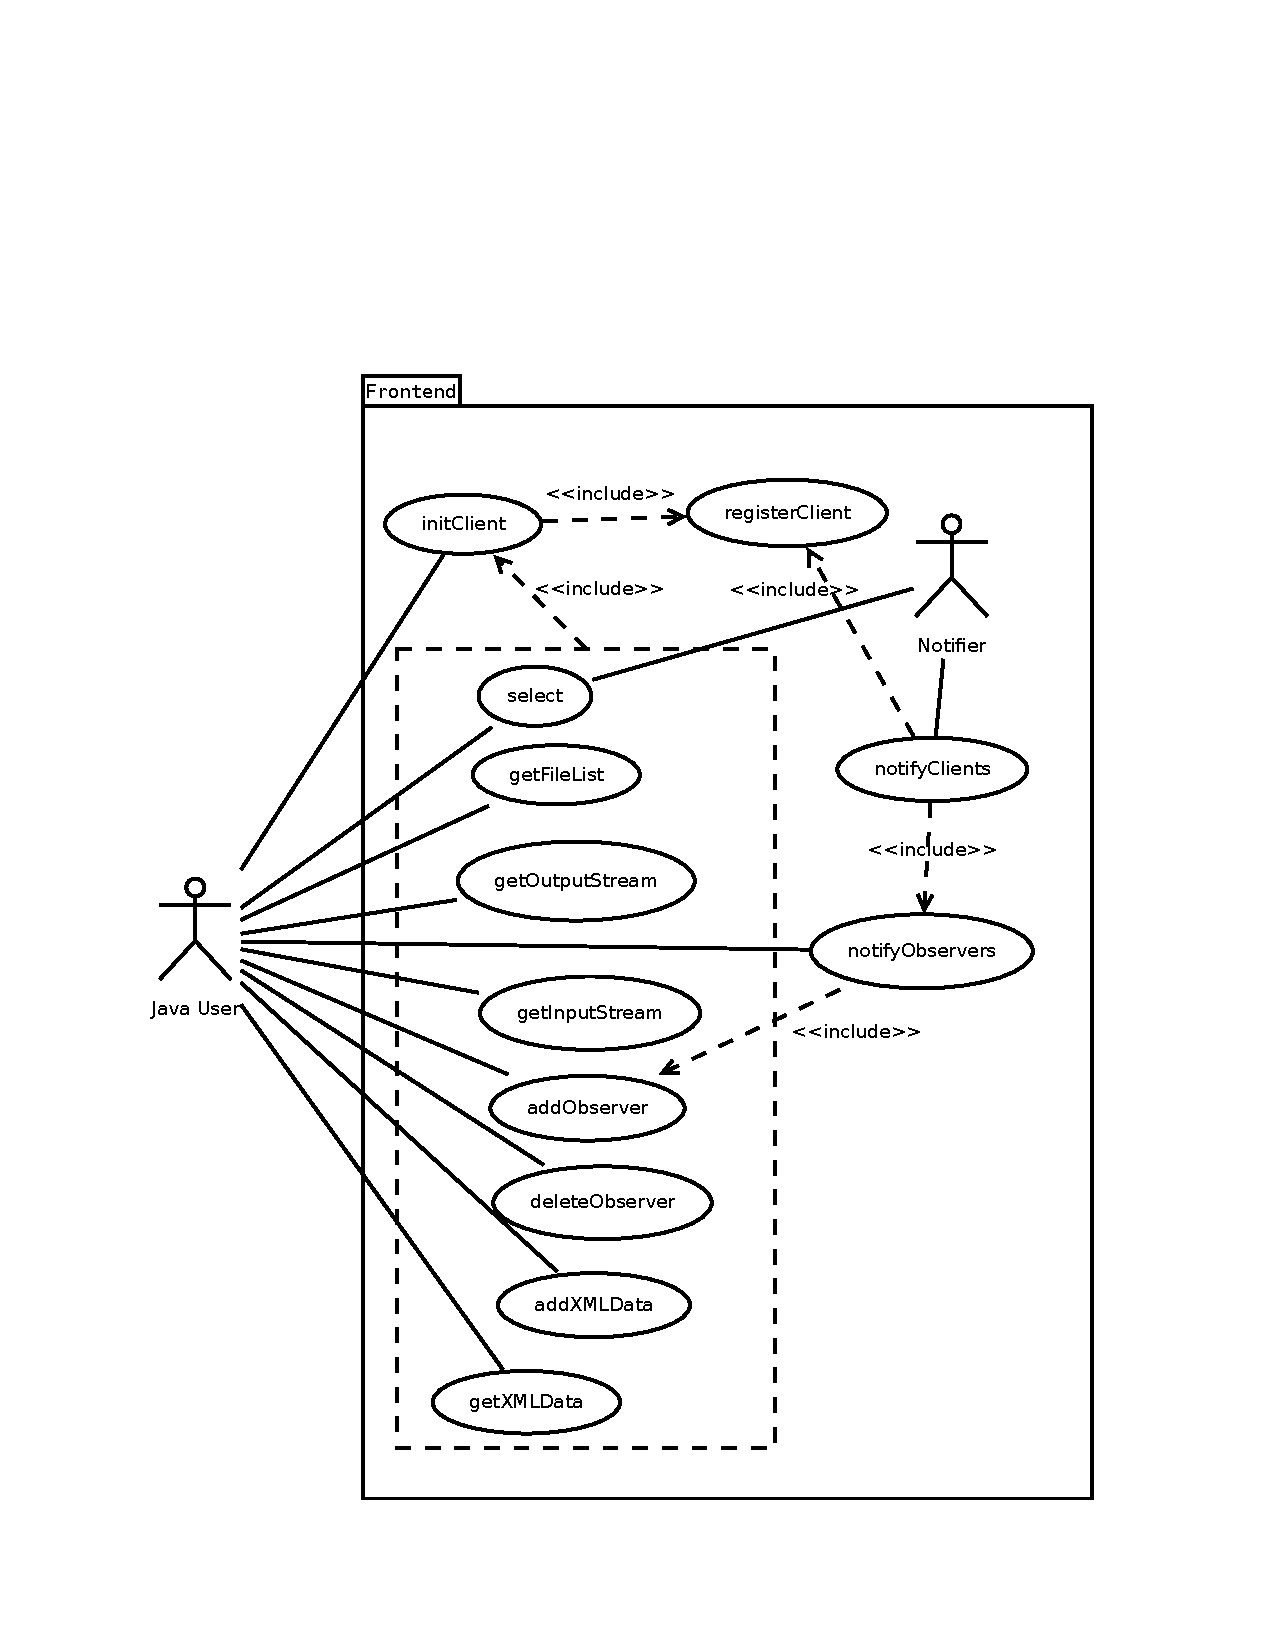
\includegraphics[height=0.9\textheight]{design/frontend/usecase.pdf}
	\caption{Diagramm: Use-Cases - Client und Server}
\end{figure}

\subsection{Java User} \label{design:frontend:usecase:user}
Java User stellen alle Akteure dar die den Client in ihr Programm einbinden. 

\begin{description}
	\item [initClient und registerClient]
		\ref{req:Cl:register}, \ref{req:Sv:register}
		beim starten des Client meldet sich dieser beim Server und wird dort registriert.
		Beendet sich ein Client so wird er aus der Registrierung genommen \ref{req:Sv:rmClients}
	\item [select]
		\ref{req:Cl:dbquery}, \ref{req:Sv:comm:dbquery} \\
		über vorbereite sql-select Schnittstellen können MetaDatenobjekte aus der
		Datenbank abgefragt werden.
	\item [getFileList]
		\ref{req:Cl:ls} \\
		Es wird eine Dateiliste eines \arc-Verzeichnisses zurückgegeben.
	\item [getOutputStream]
		\ref{req:Cl:writeFile} \\
		Es wird ein Outputstream zurückgegeben um Dateien in das Archiv zu schreiben.
	\item [getInputStream]
		\ref{req:Cl:readFile} \\
		Über einen Inputstream können aus dem Archiv gelesen werden.
	\item [getXMLData]
		\ref{req:Cl:selectTag} \\
		Es werden bestimmte XML-Daten zurückgegeben.
	\item [addXMLData]
		\ref{req:Cl:addTag} \\
		Es können neue Elemente zu den XML-Daten hinzugefügt werden.
	\item [add / deleteObserver]
		\ref{req:Cl:observer}, \ref{req:Cl:notifies} \\
		Es können Observer an- und abgemeldet werden, welche Update-daten aus dem
		Archiv bekommen können.
\end{description}

\section{API}
Neben den in Abschnitt \ref{design:data:classes} beschriebenen Datenklassen enthält die
API noch folgende Klassen und Interfaces:
\begin{description}
	\item [WebarchiveClientFactory]
		Die Factory bietet Möglichkeiten zur Konfiguration und Erzeugung der Clients
	\item [WebarchiveClient]
		Der WebarchiveClient ist die Zentrale Programmierschnittstelle an das Webarchiv.
		Es lassen sich Aktionen wie unter Abschnitt \ref{design:frontend:usecase:user} ausführen.
	\item [XmlEdit]
		Hilfsklasse zum Bearbeiten der XML-Dateien.
	\item [WebarchiveObserver]
		Implementierer dieser Schnittstelle werden über Updates benachrichtigt.
\end{description}
Details zeigt Diagramm \ref{dia:design:frontend:cl:api}
\begin{figure}[!h]
	\centering
	\label{dia:design:frontend:cl:api}
	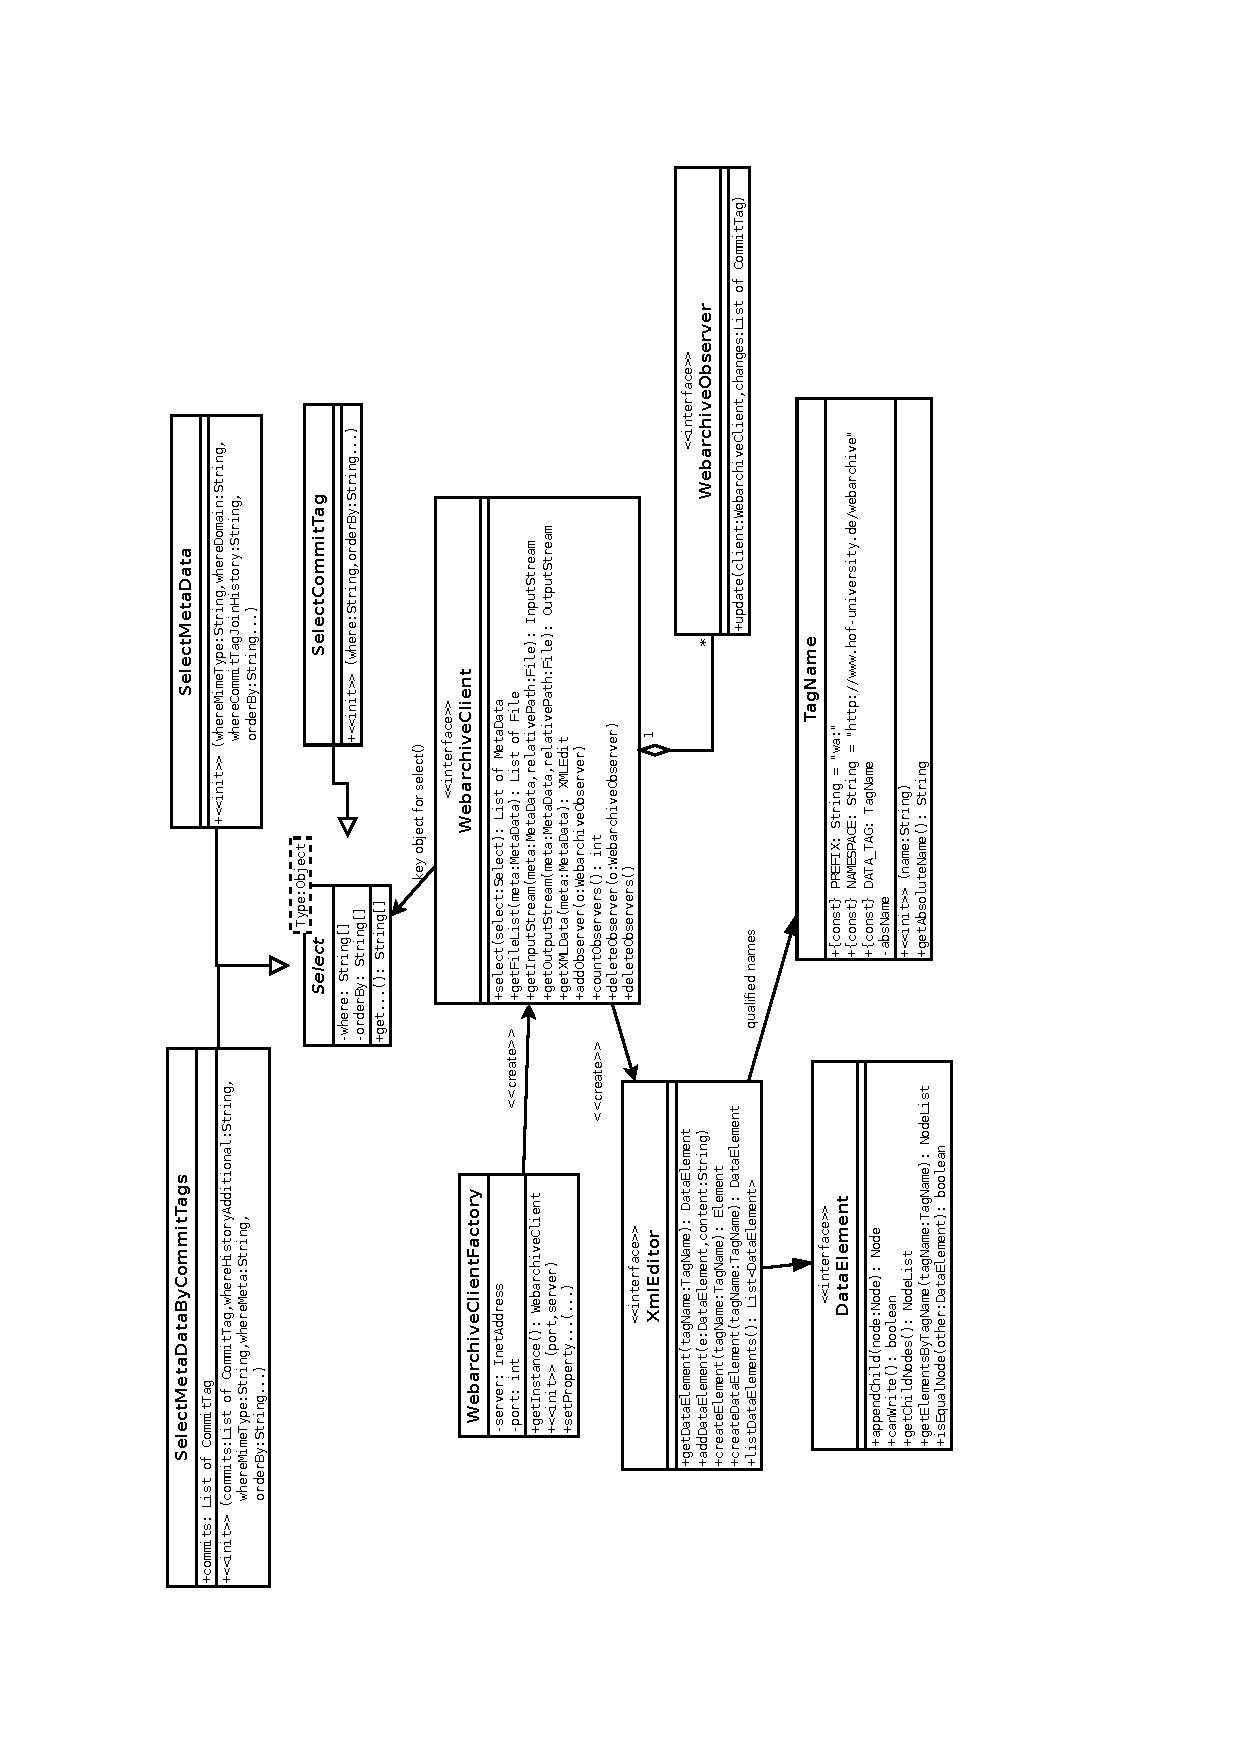
\includegraphics[angle=270, width=1.1\textwidth]{design/frontend/classes/api-Klassen.pdf}
	\caption{Klassendiagramm: API}
\end{figure}

\section{Programmfluss}

Verantwortlich: Eduard Schneider

Alle Client$\rightarrow$Server Kommunikationen basieren auf dem gleichen Schema.

Nachdem der Analyzer eine Methode der API aufgerufen hat, wird zunächst ein Message-Datenobjekt mit dem zum Aufruf passenden Header auf Client-Seite angelegt.

Anschließend wird dieses Objekt an den Server gesendet und geprüft, welche Aktion vom Server ausgeführt werden soll.
Bei Anfragen, die eine Antwort vom Server erwarten, wird die Message noch mit einer ID-Nummer markiert und in eine Map im Client eingetragen und der aufrufende Thread der API-Methode schlafend gelegt.
Über diese ID wird bei einer Antwort vom Server der schlafende Thread geweckt und mit der Antwort verknüpft.


Wenn die auszuführende Aktion einen Schreib- oder Lesezugriff auf das Archiv bedeutet, wird diese mit einer Lock- und Unlock-Sequenz eingeschlossen.
Sobald der Server die Aufgabe erledigt und eventuelle Locks freigegeben hat, wird ein neues Message-Objekt auf Serverseite erzeugt und an den Client gesendet und ausgwertet.
Sie kann Daten, Benachrichtigungen über den Erfolg der Aufgabe oder Exceptions enthalten.

\subsection {select}

Das Auslesen von MetaDaten aus der Datenbank ist kein auf das Archiv lesender oder schreibender Ablauf, sodass hier auf ein Locken oder Unlocken verzichtet werden kann, bzw. durch das DBMS erfolgt.

select() entspricht der einfachsten Form der Client$\rightarrow$Server Kommunikation.
Hier wird das, durch die eigene Implementierung der select()-Methode vorgefertigte SQL-Statement nur an die dbSelect-Sequenz durchgereicht, welche eine Liste aus MetaDaten zurückliefert.
Die Liste kann dann an den Client zurückgesendet und schließlich dem Analyzer vorgelegt werden.

\begin{figure}[H]
	\centering
	\label{dia:design:frontend:sqc:select}
	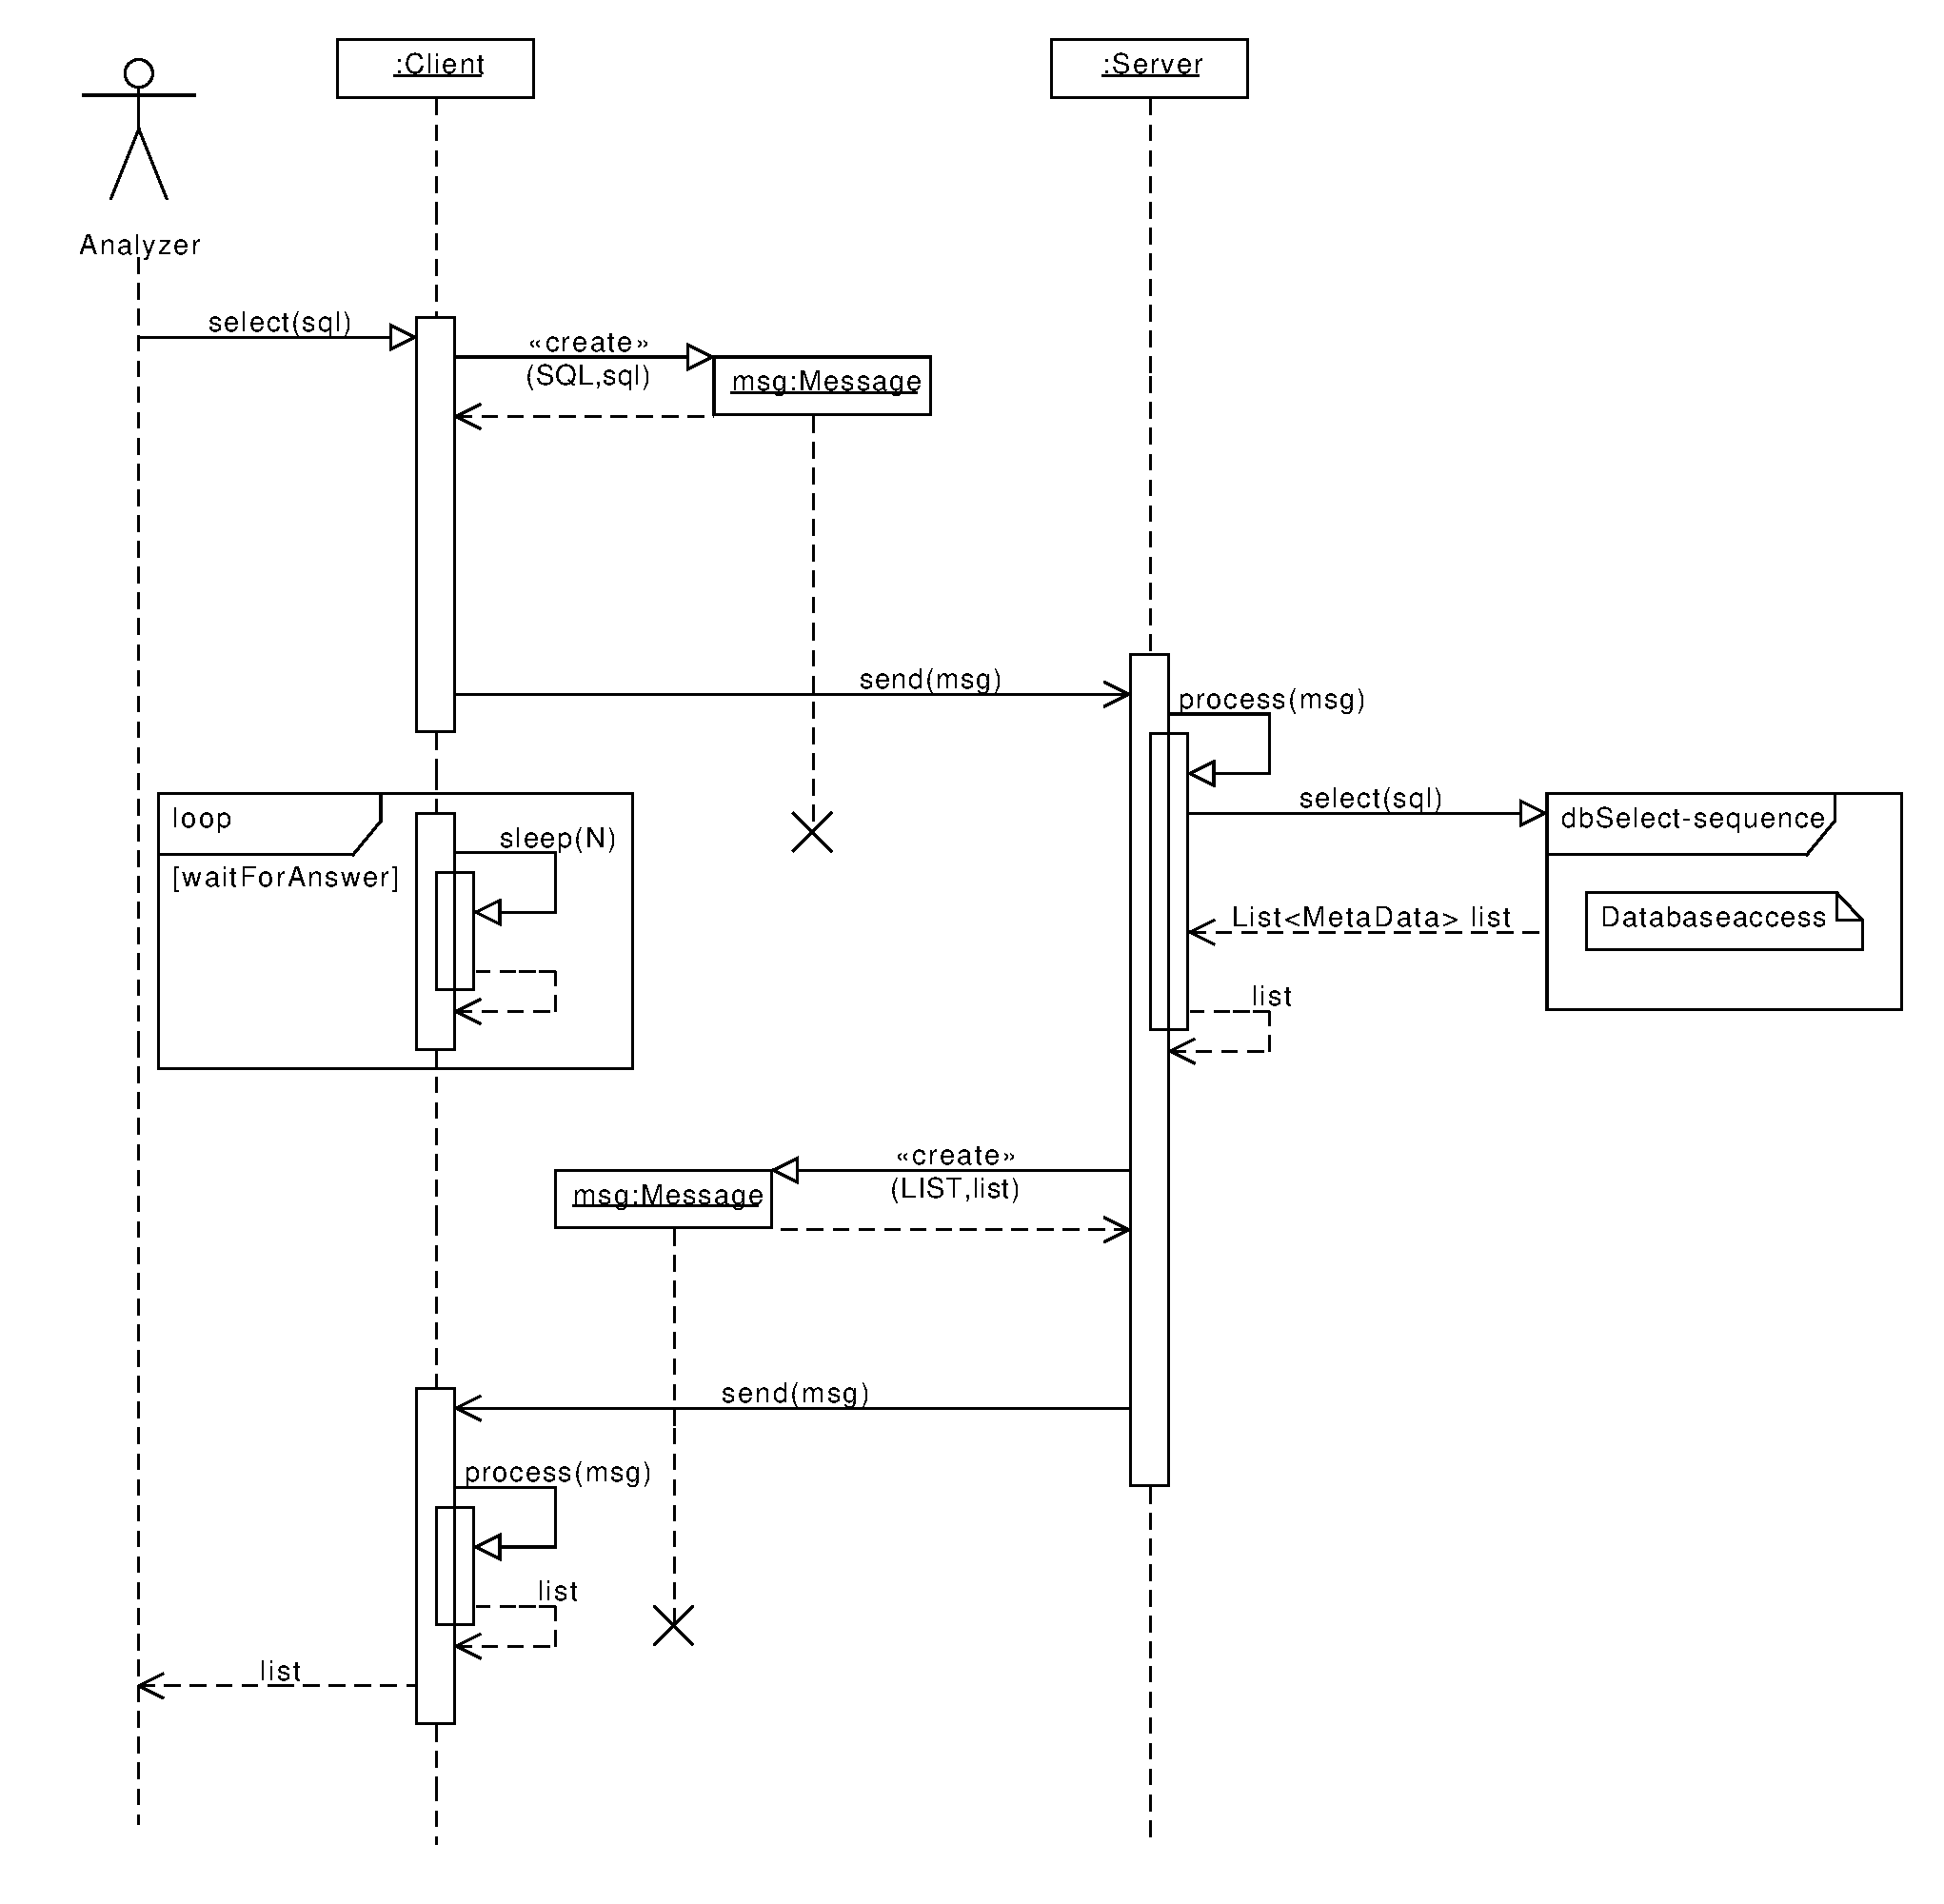
\includegraphics[width=\textwidth]{design/frontend/sequence/select-sequence.pdf}
	\caption{Sequenzdiagramm: Select}
\end{figure}

\subsubsection{Lock setzen}

Bei Schreib- und Lesezugriffen auf das Archiv wird ein Datei-Mutex gesetzt.

Die Lock-Sequenz fragt beim Python-Lock-Modul einen Mutex in einem bestimmten Domain-Ordner an.

Ist dieser Ordner bereits gesperrt, blockiert das Python-Modul solange bis der Lock erfolgreich oder eine Zeitgrenze überschritten wurde.
Bei letzterem wird eine Exception erzeugt und an den Client weitergegen.
Wenn keine Probleme aufgetreten sind, kann noch gegebenenfalls eine Checkout-Anfrage durch das selbe Prinzip gestellt werden.
Die Sequenz muss also über die Fähigkeit verfügen, Textnachrichten an das Python-Modul schicken und empfangen zu können.

%\begin{figure}[h]
%	\centering
%	\label{dia:design:frontend:sqc:lock}
%	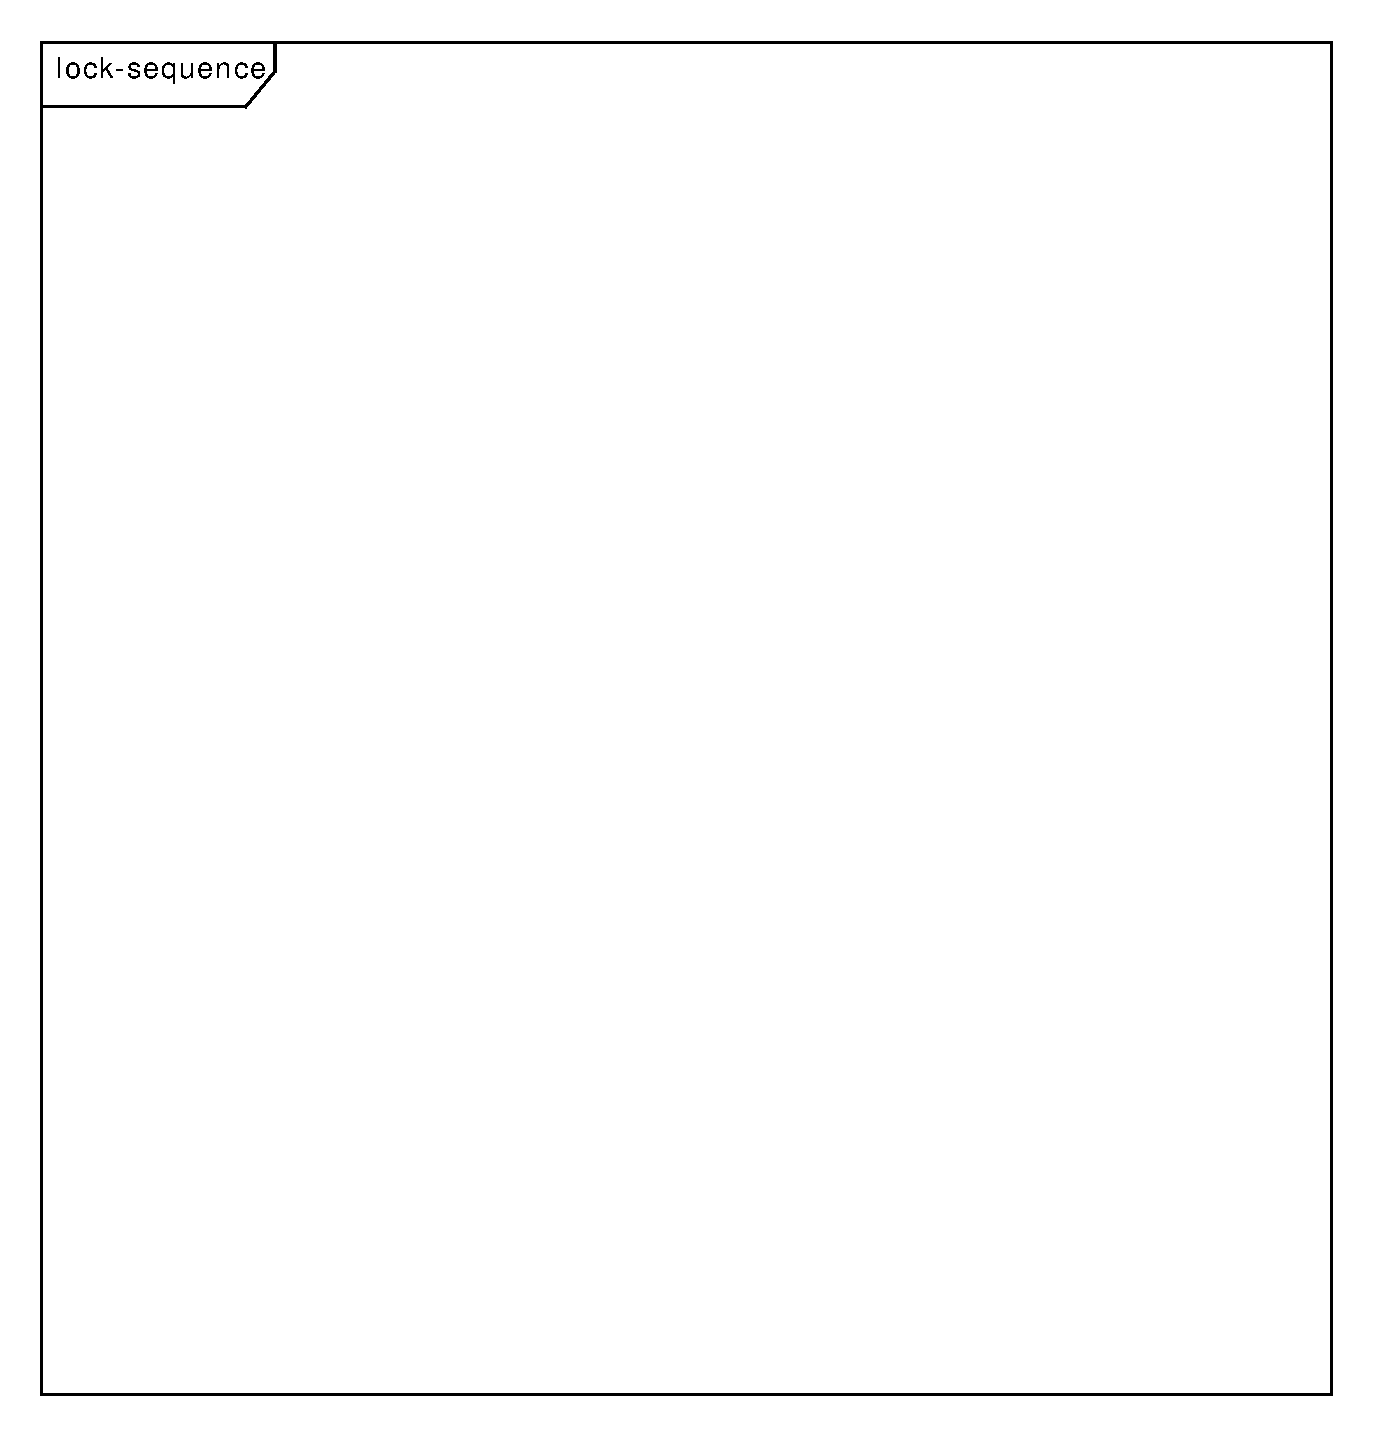
\includegraphics[width=0.5\textwidth]{design/frontend/sequence/lock-sequence.pdf}
%	\caption{Sequenzdiagramm: Lock setzen}
%\end{figure}

\subsubsection{Unlock}

Das Unlocken entspricht bis auf die Textnachrichten dem gleichen Prinzip wie das Locken.
%\begin{figure}[h]
%	\centering
%	\label{dia:design:frontend:sqc:unlock}
%	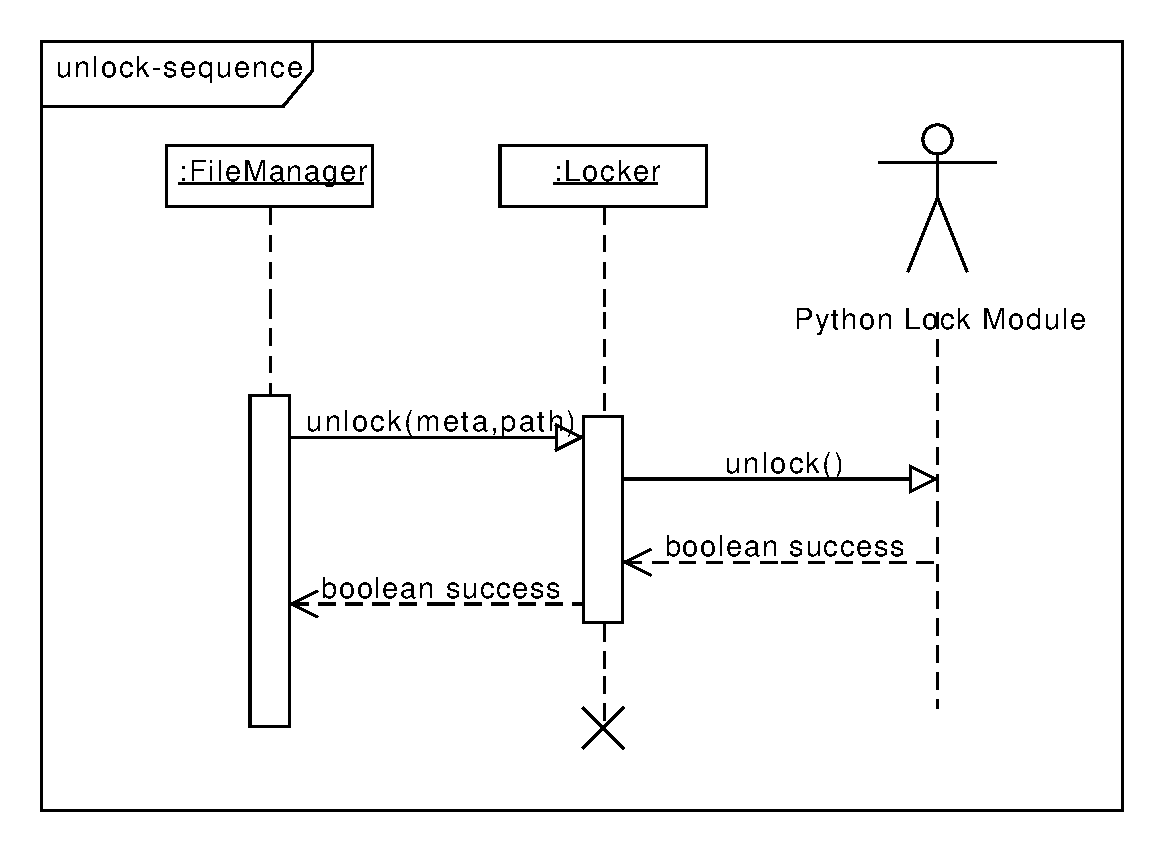
\includegraphics[width=0.5\textwidth]{design/frontend/sequence/unlock-sequence.pdf}
%	\caption{Sequenzdiagramm: Unlock}
%\end{figure}


\subsection {getOutputStream}

Um eine Analyse-Datei in das Archiv schreiben zu können, stellt der Client einen speziellen ByteArrayOutputStream (BAOS) zur Verfügung.
Dieser kann vom Analyzer wie ein normaler OutputStream genutzt werden.
Werden Daten in den Stream geschrieben, landen sie in einem internen byte[]-Puffer des BAOS.

Führt der Analyzer die eigens implementierte close()-Methode aus, setzt er die Leerung des BAOS in das erzeugte Buffer-Objekt und das Senden des Buffers an den Server in Gang.

Auf der Serverseite wird nach der Verarbeitung der Nachricht, ein Lock gesetzt und versucht die Daten des Buffer-Objekts in das Archiv zu schreiben.
Anschließend wird der Lock entfernt, eine ,,SUCCESS''-Nachricht an den Client geschickt und die close()-Methode beendet.

\begin{figure}[H]
	\centering
	\label{dia:design:frontend:sqc:getOutputStream}
	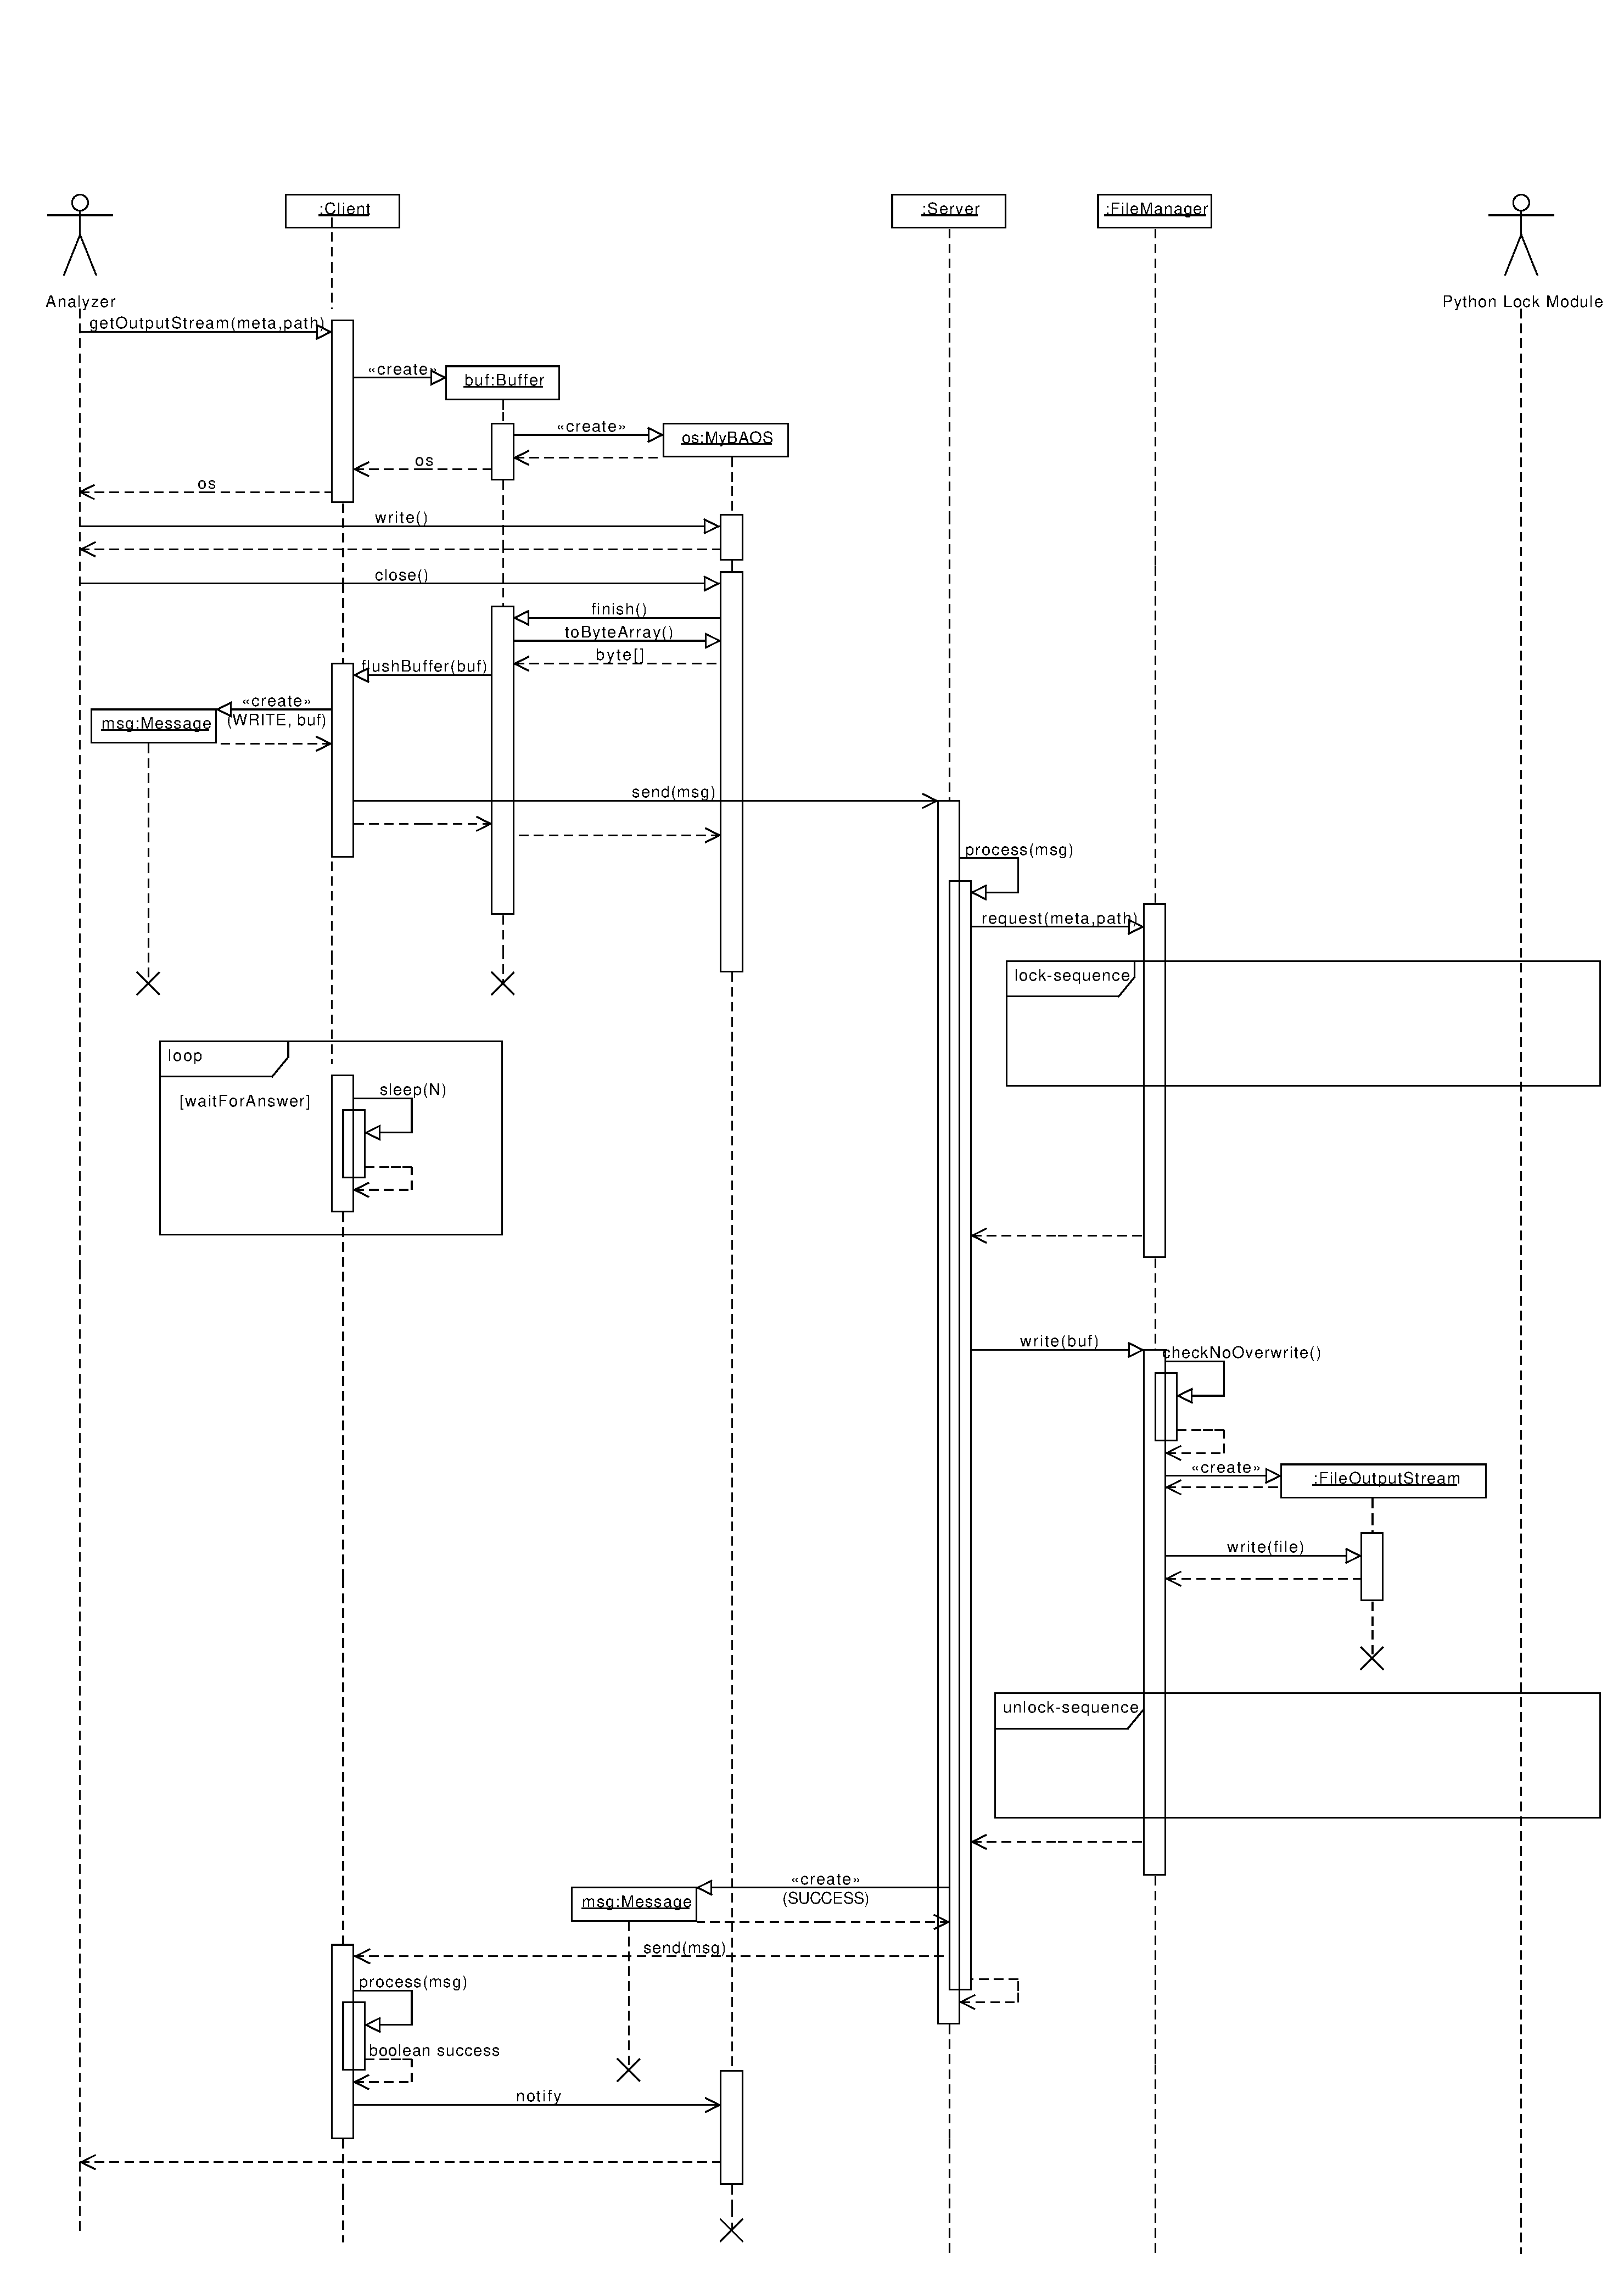
\includegraphics[width=\textwidth]{design/frontend/sequence/get-output-stream-sequence.pdf}
	\caption{Sequenzdiagramm: getOutputStream}
\end{figure}

\subsection {getInputStream}

Um eine beliebige Datei aus dem Archiv zu lesen, wird ein FileDescriptor der zu lesenden Datei an den Server geschickt.
Nach erfolgreichem Locken erzeugt der Server ein Buffer-Objekt mit der Datei als Inhalt und schickt es an den Client.
Dieser erstellt einen ByteArrayInputStream(BAIS) mit Hilfe der Daten im Buffer-Objekt und gibt den BAIS nach Unlocken  an den Analyzer zurück.
Der BAIS kann genau wie jeder andere Stream genutzt werden.

\begin{figure}[H]
	\centering
	\label{dia:design:frontend:sqc:getInputStream}
	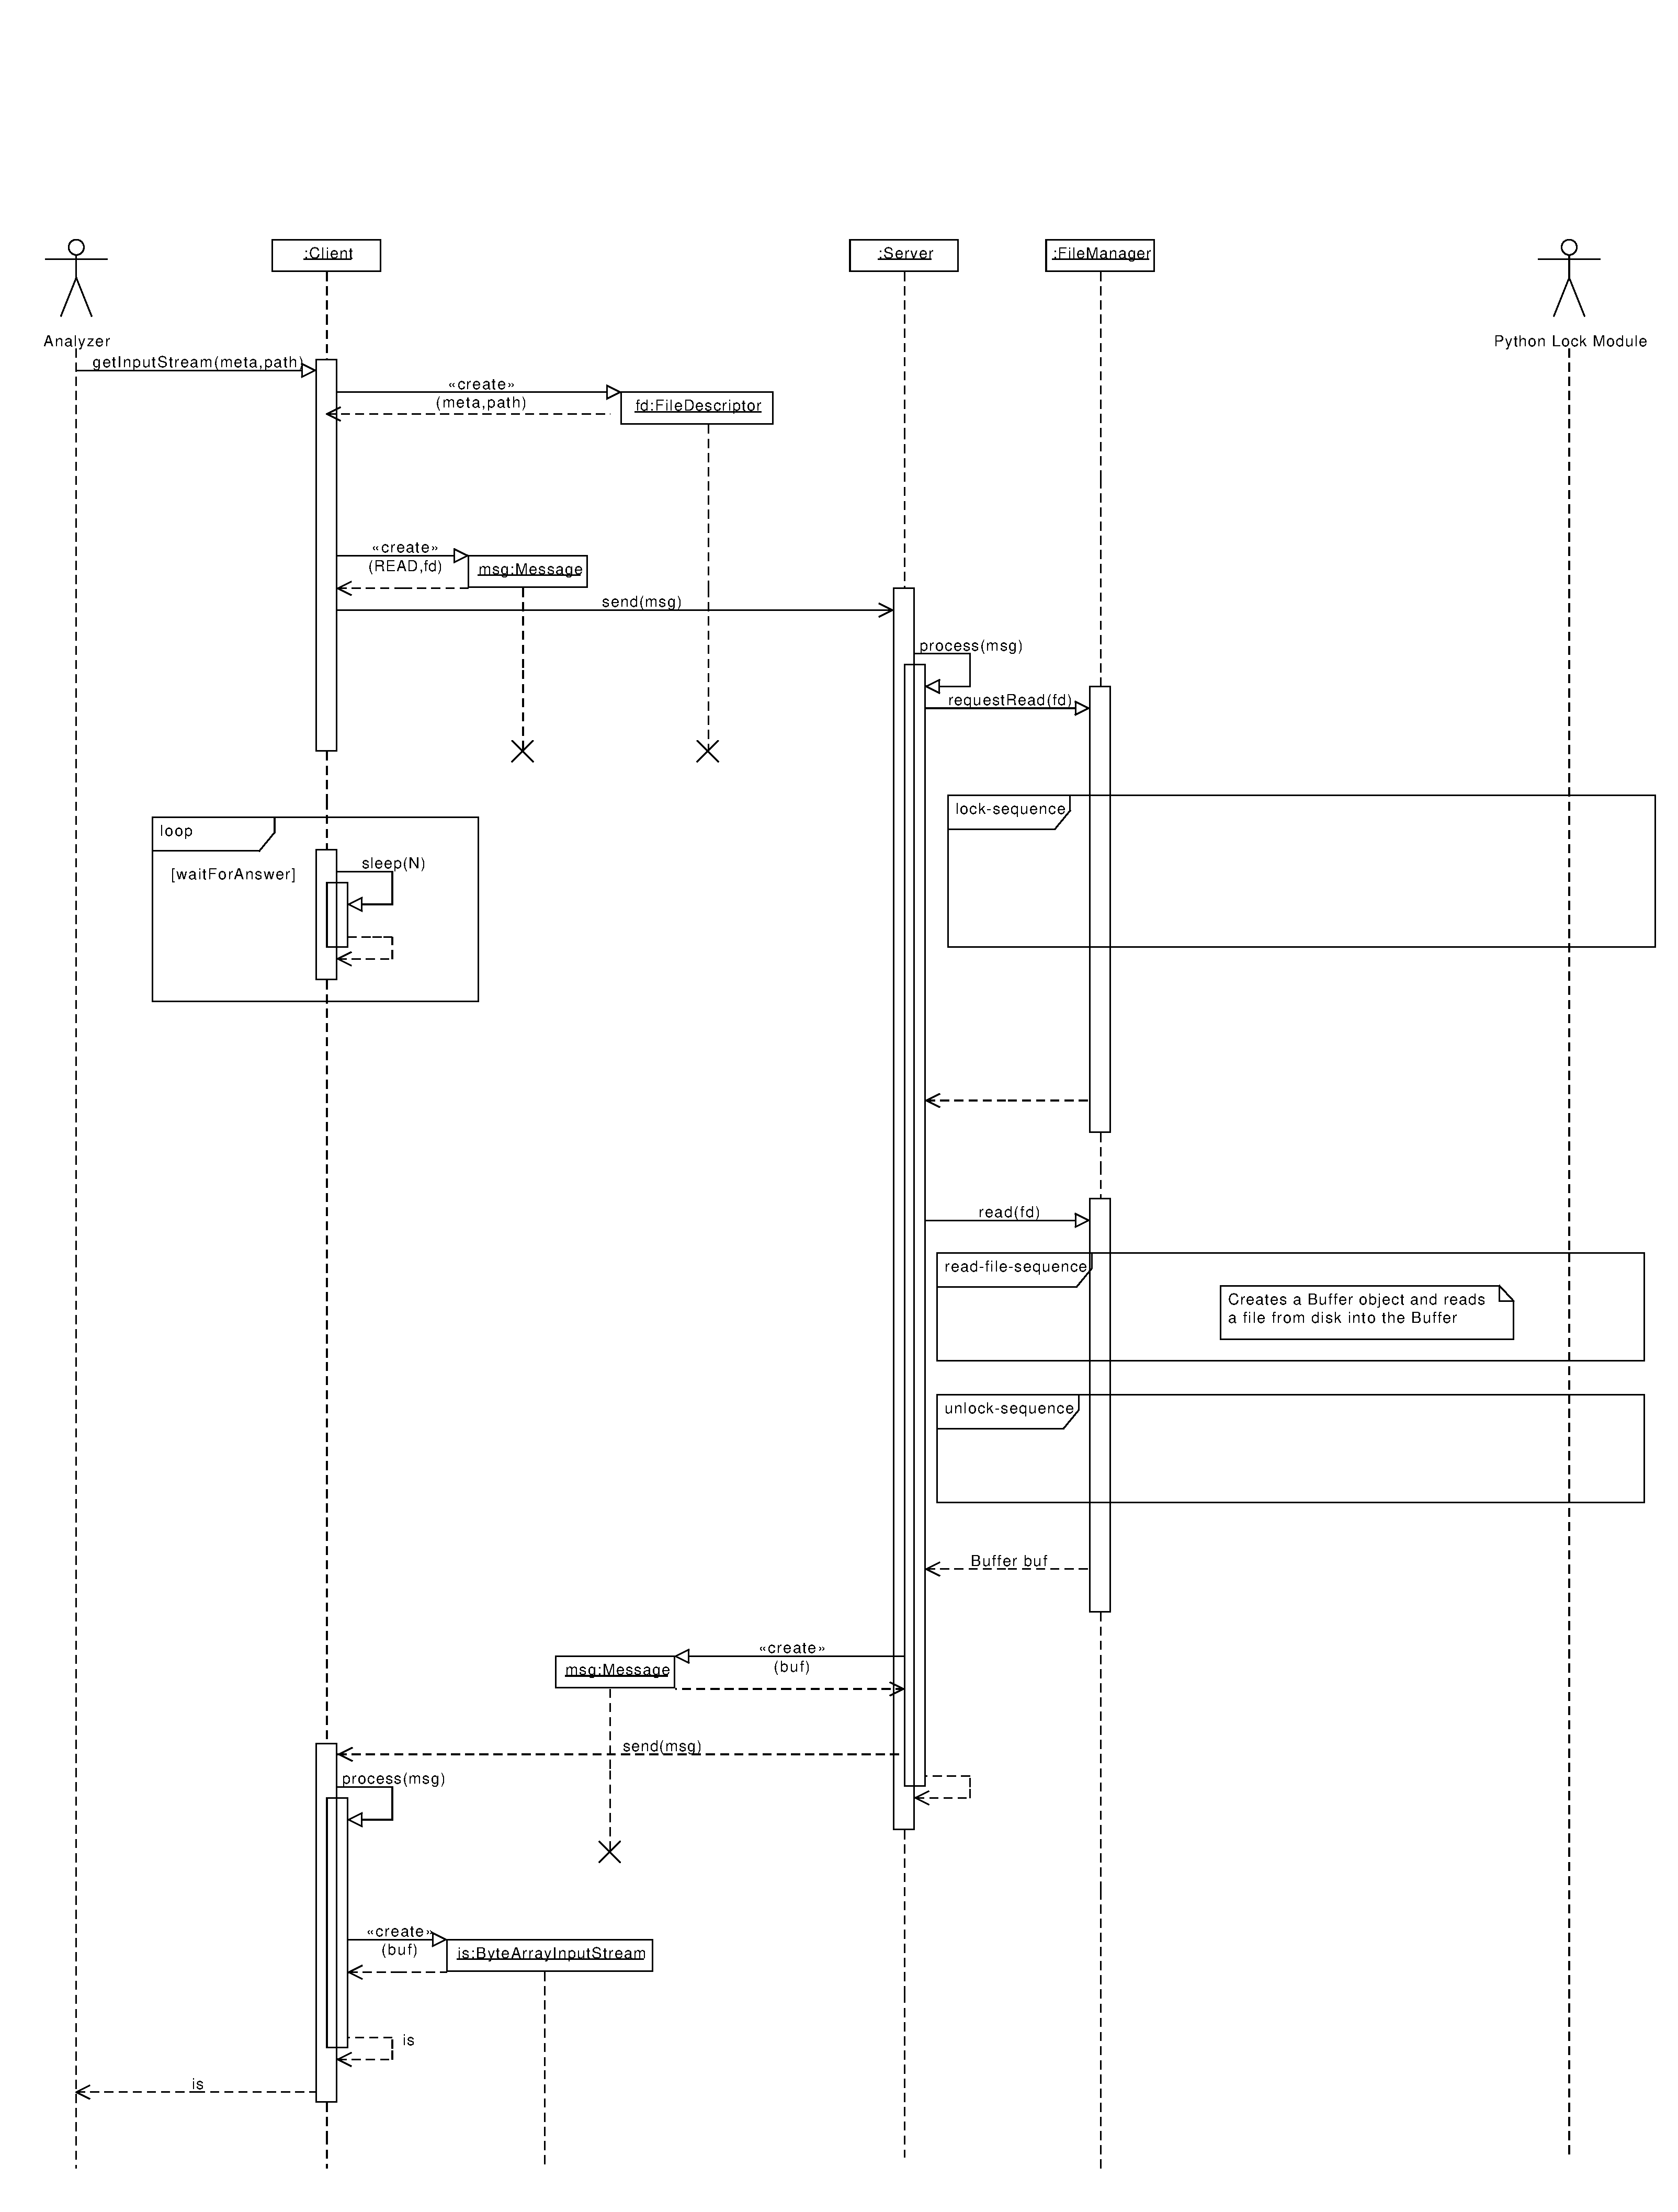
\includegraphics[width=\textwidth]{design/frontend/sequence/get-input-stream-sequence.pdf}
	\caption{Sequenzdiagramm: getInputStream}
\end{figure}




\subsection {getXMLData}


Analog zu den bisherigen Kommunikationsdiagrammen wird beim Lesen von XML-Dateien zuerst eine Anfrage in Form einer Message an den Server gesendet.
Nachdem der Server liest die XML-Datei nach dem locken aus und sendet den Inhalt an den Client.
Dieser gibt die XML-Datei jedoch nicht direkt an den Analyzer zurück, sondern erstellt mit den Daten eine Instanz der Klasse XMLEdit.
Nachdem XMLEdit an den Analyzer übergeben wurde, kann er beliebige XML-Elemente mit dem XMLEdit ausgeben lassen.

%\begin{figure}[h]
%	\centering
%	\label{dia:design:frontend:sqc:select}
%	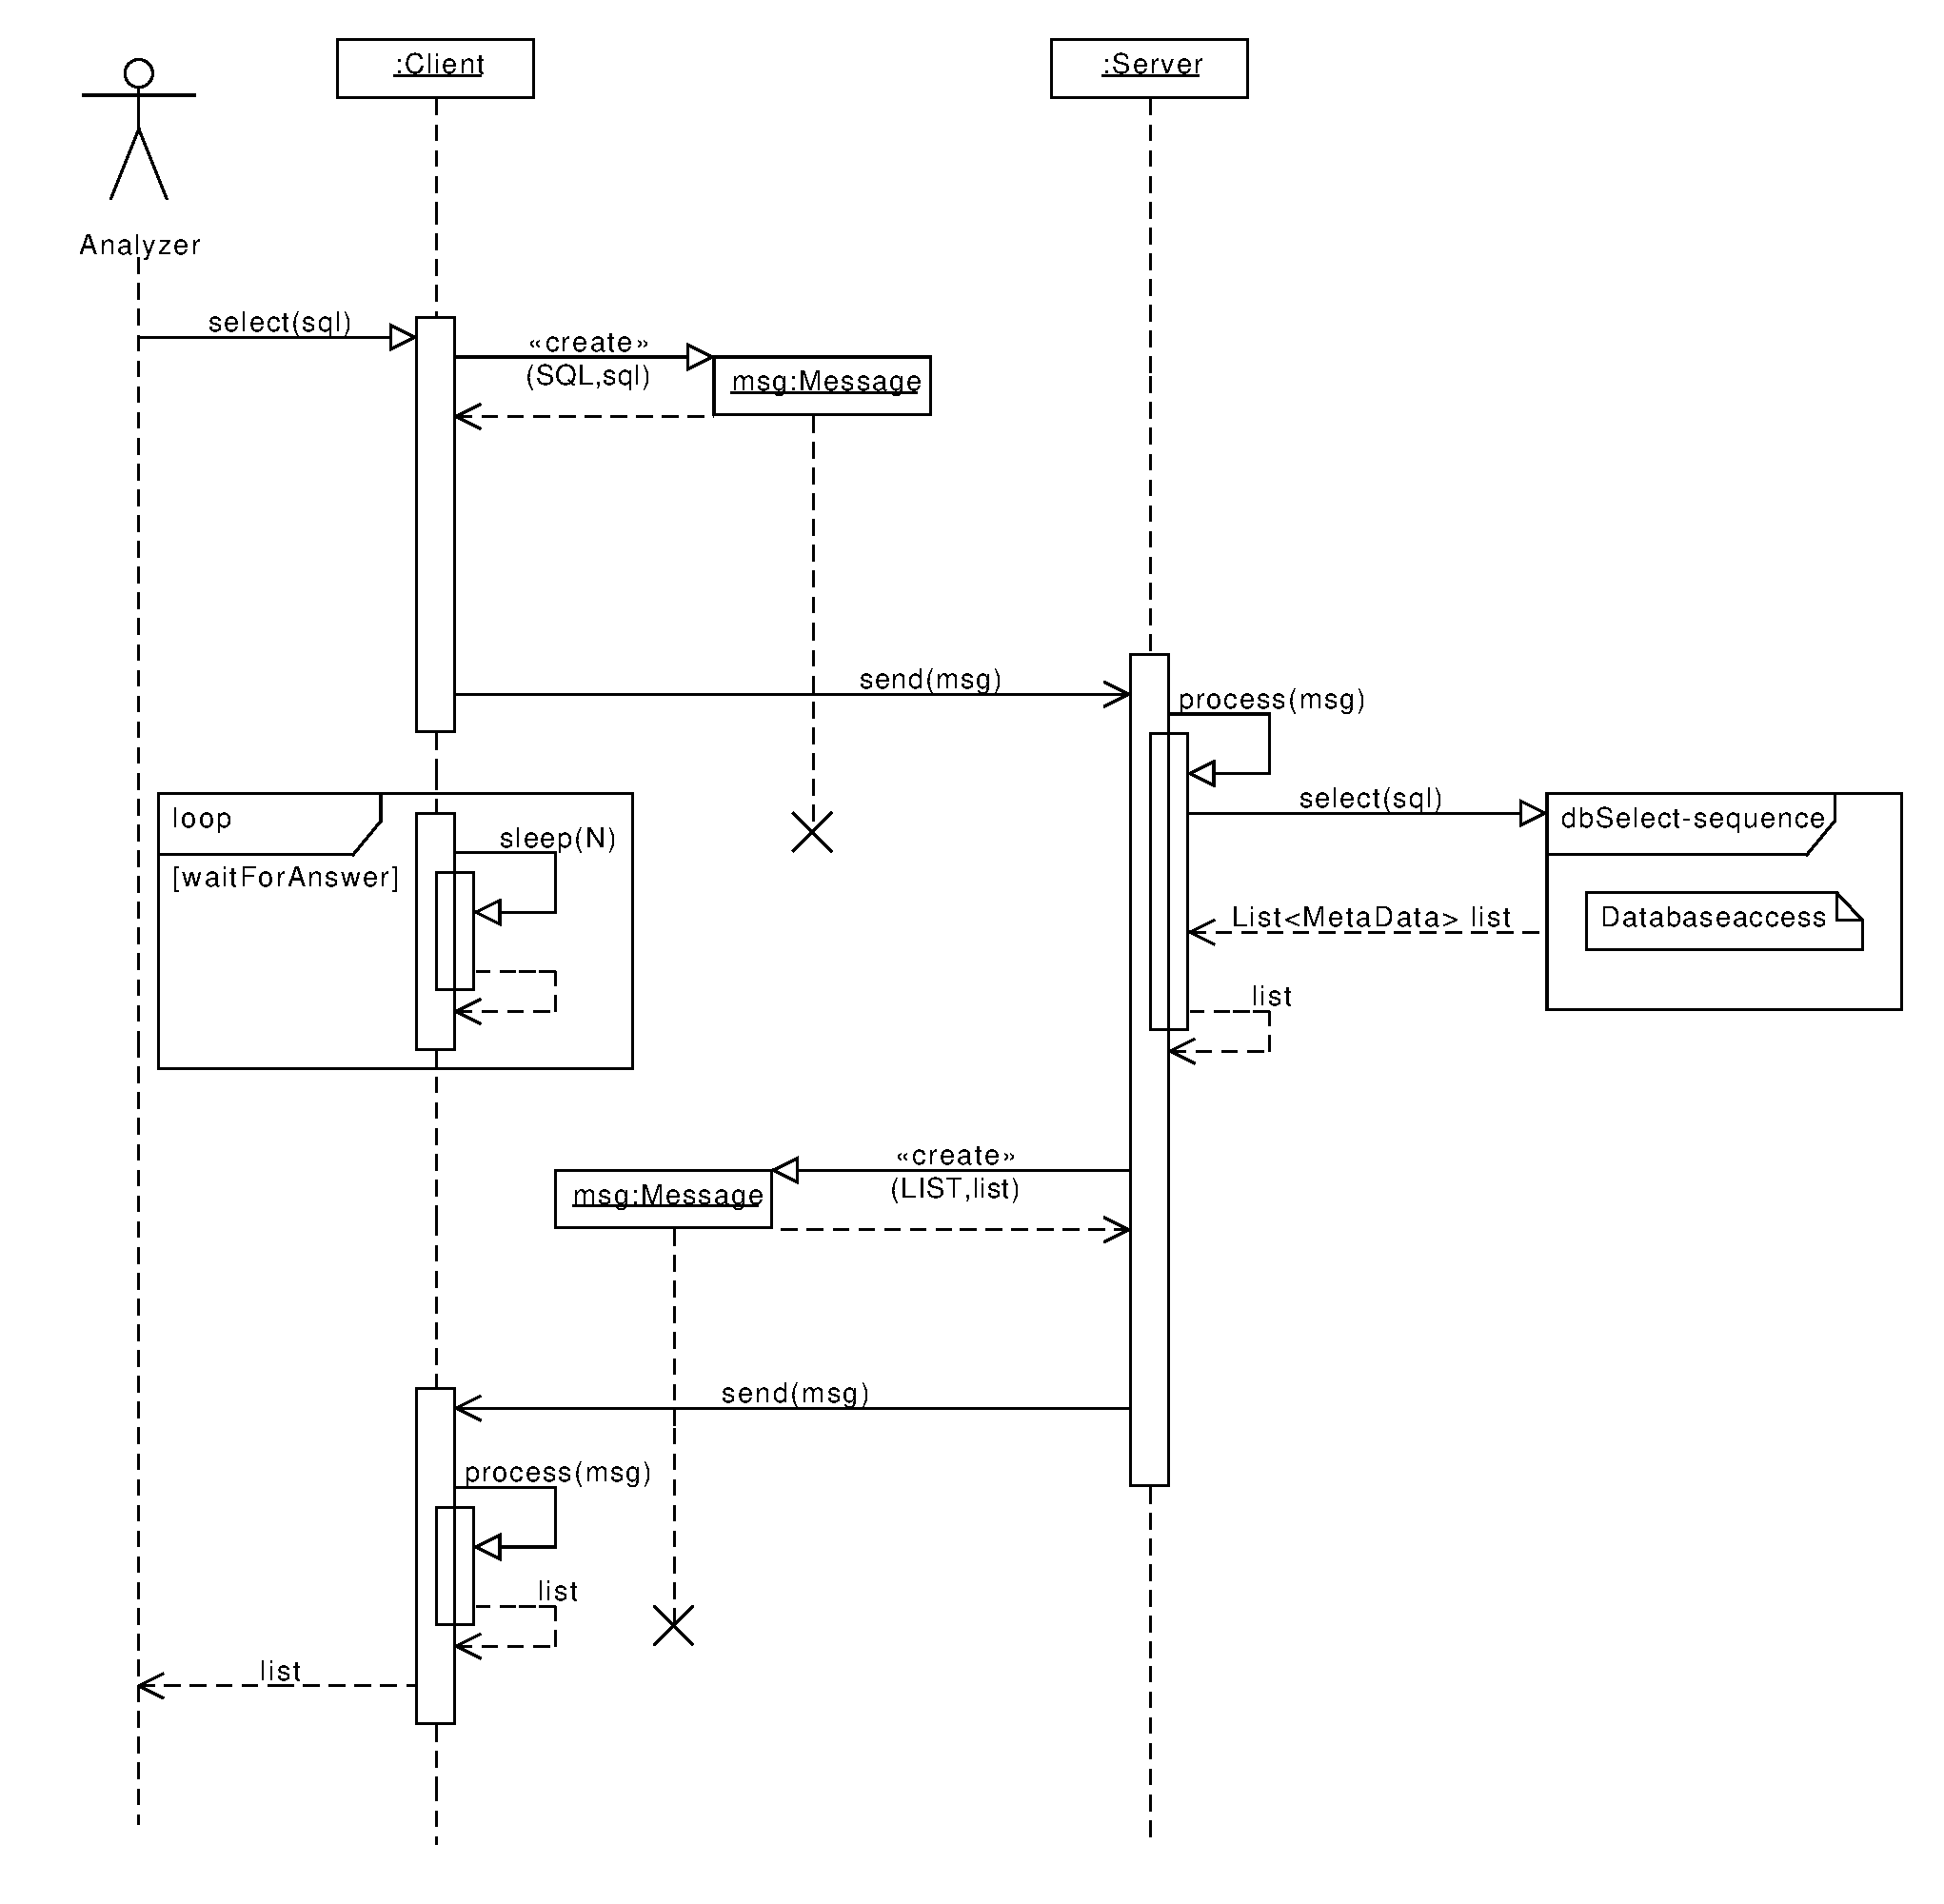
\includegraphics[width=\textwidth]{design/frontend/sequence/select-sequence.pdf}
%	\caption{Sequenzdiagramm: Select}
%\end{figure}

\subsection {addXMLData}

XML-Daten lassen sich nicht direkt über die API in das Archiv schreiben, sondern müssen mithilfe der XMLEdit-Klasse erzeugt werden.
Dazu wird zuerst getXMLData() aufgerufen, um eine Kopie der zu bearbeitenden XML-Datei zu erhalten.
Anschließend kann mit addNode() ein neues Element hinzugefügt  werden.
addNode() schickt dann eine Nachricht mit dem neuen Element an den Server.
Dieser baut das neue Element in die XML-Datei ein.
Bereits vorhandene Elemente können nicht gelöscht oder überschrieben werden.
Diese Vorgehensweise bietet dem Analyzer einfache Methoden, um XML-Elemente für Analsyse-Daten zu erzeugen.

%\begin{figure}[h]
%	\centering
%	\label{dia:design:frontend:sqc:select}
%	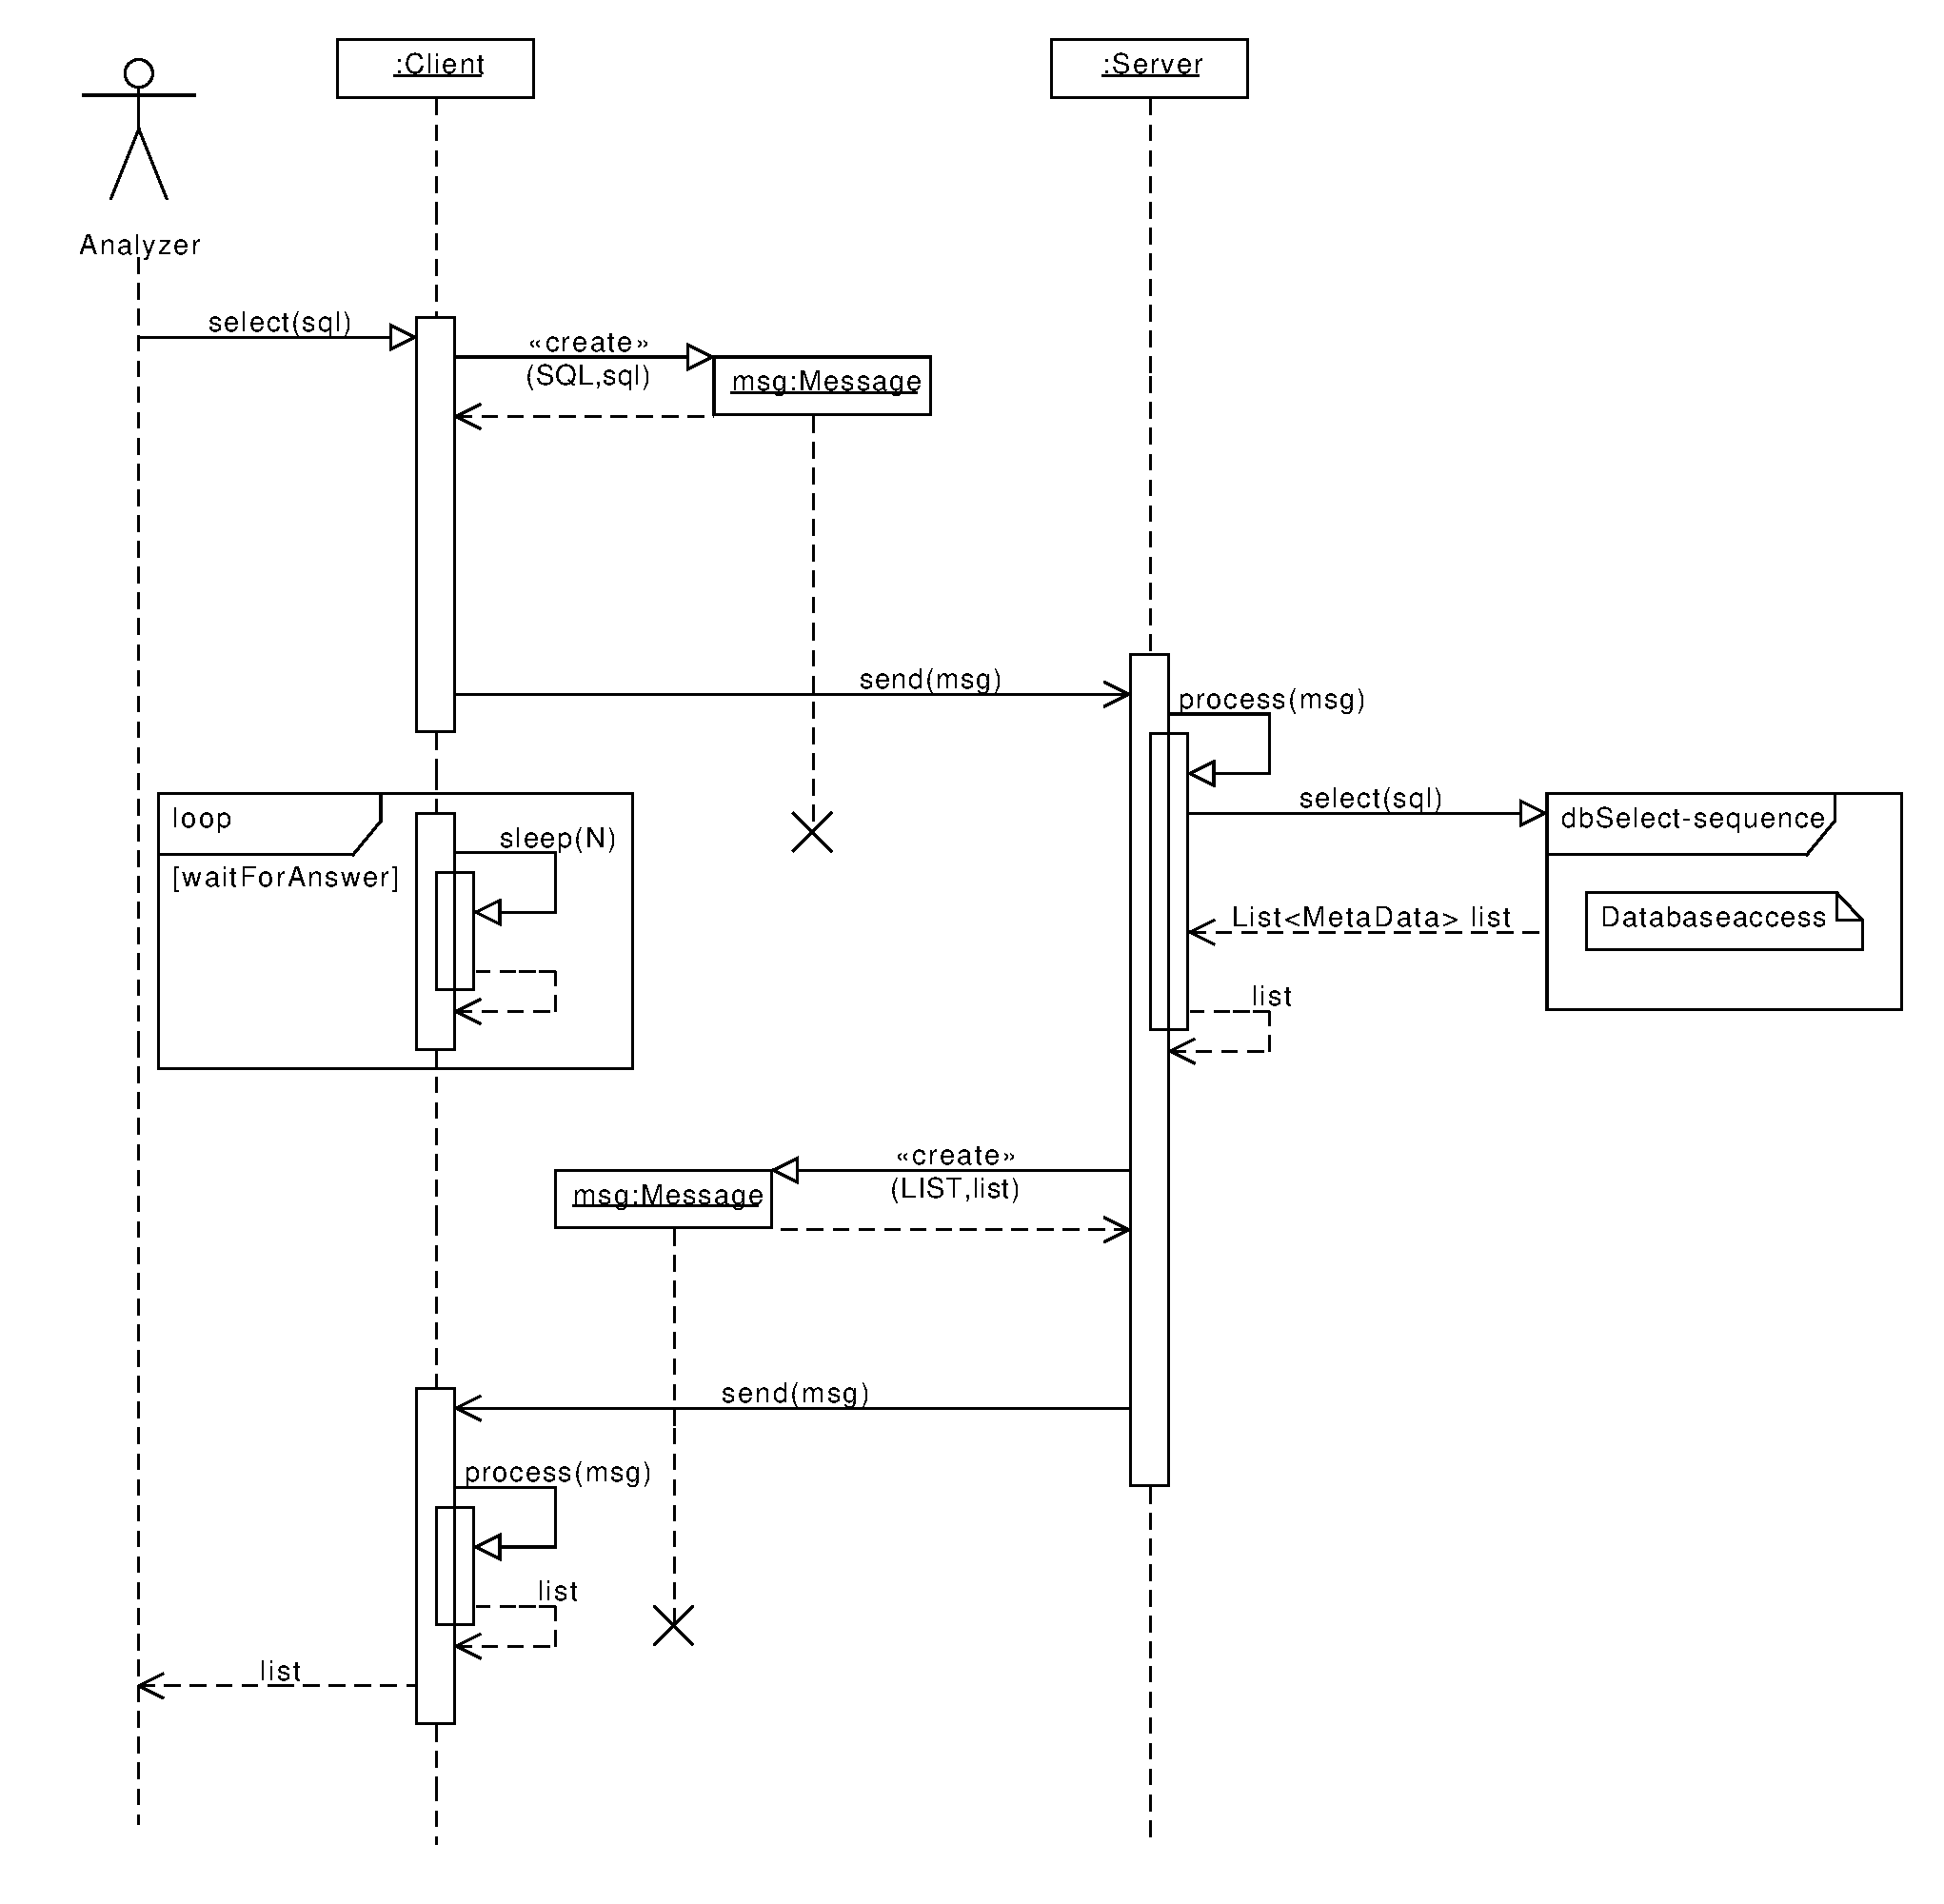
\includegraphics[width=\textwidth]{design/frontend/sequence/select-sequence.pdf}
%	\caption{Sequenzdiagramm: Select}
%\end{figure}

\subsection {add / deleteObserver}

Um vom Server über neue Versionen oder sogar neue Webseiten automatisch informiert zu werden, kann sich der Client am Server als Observer anmelden.
Gleichzeitig meldet sich der Analyzer über die Java eigene Observer Implementierung am Client als Observer an.
Beides geschieht über den Aufruf der API-Methode addObserver(Observer).
Sobald sich der Analyzer anmeldet, wird auch der client im Server in eine spezielle Liste eingetragen.
Das Abmelden wird analog mit deleteObserver(Observer) realisiert.

\subsection {getFileList}

Wie die bisherigen Methoden der API.
Es wird auf Serverseite eine Liste von File-Objekten erzeugt und an den Client gesendet.
Diese kann einfach an den Analyzer zurückgegeben werden.

\section {Client Notifier}
% SABRINAS PART
Zum Benachrichtigen über Neuerungen des Webarchivs für die Observer (Clients) wird ein Notifier eingesetzt.

Dieser erhält beim Start ein Intervall, welches beschreibt, innerhalb welchen Zeitraum die Observer  benachrichtigt werden müssen. Ist das der Fall, startet ''Observerble'' die Benachrichtigungsroutine  "NotificationSequence". Sobald diese Beendet ist, legt sich der Threat  für das vorgegeben Intervall schlafen.

\begin{figure}[H]
	\centering
%	\label{dia:design:frontend:sqc:getOutputStream}
	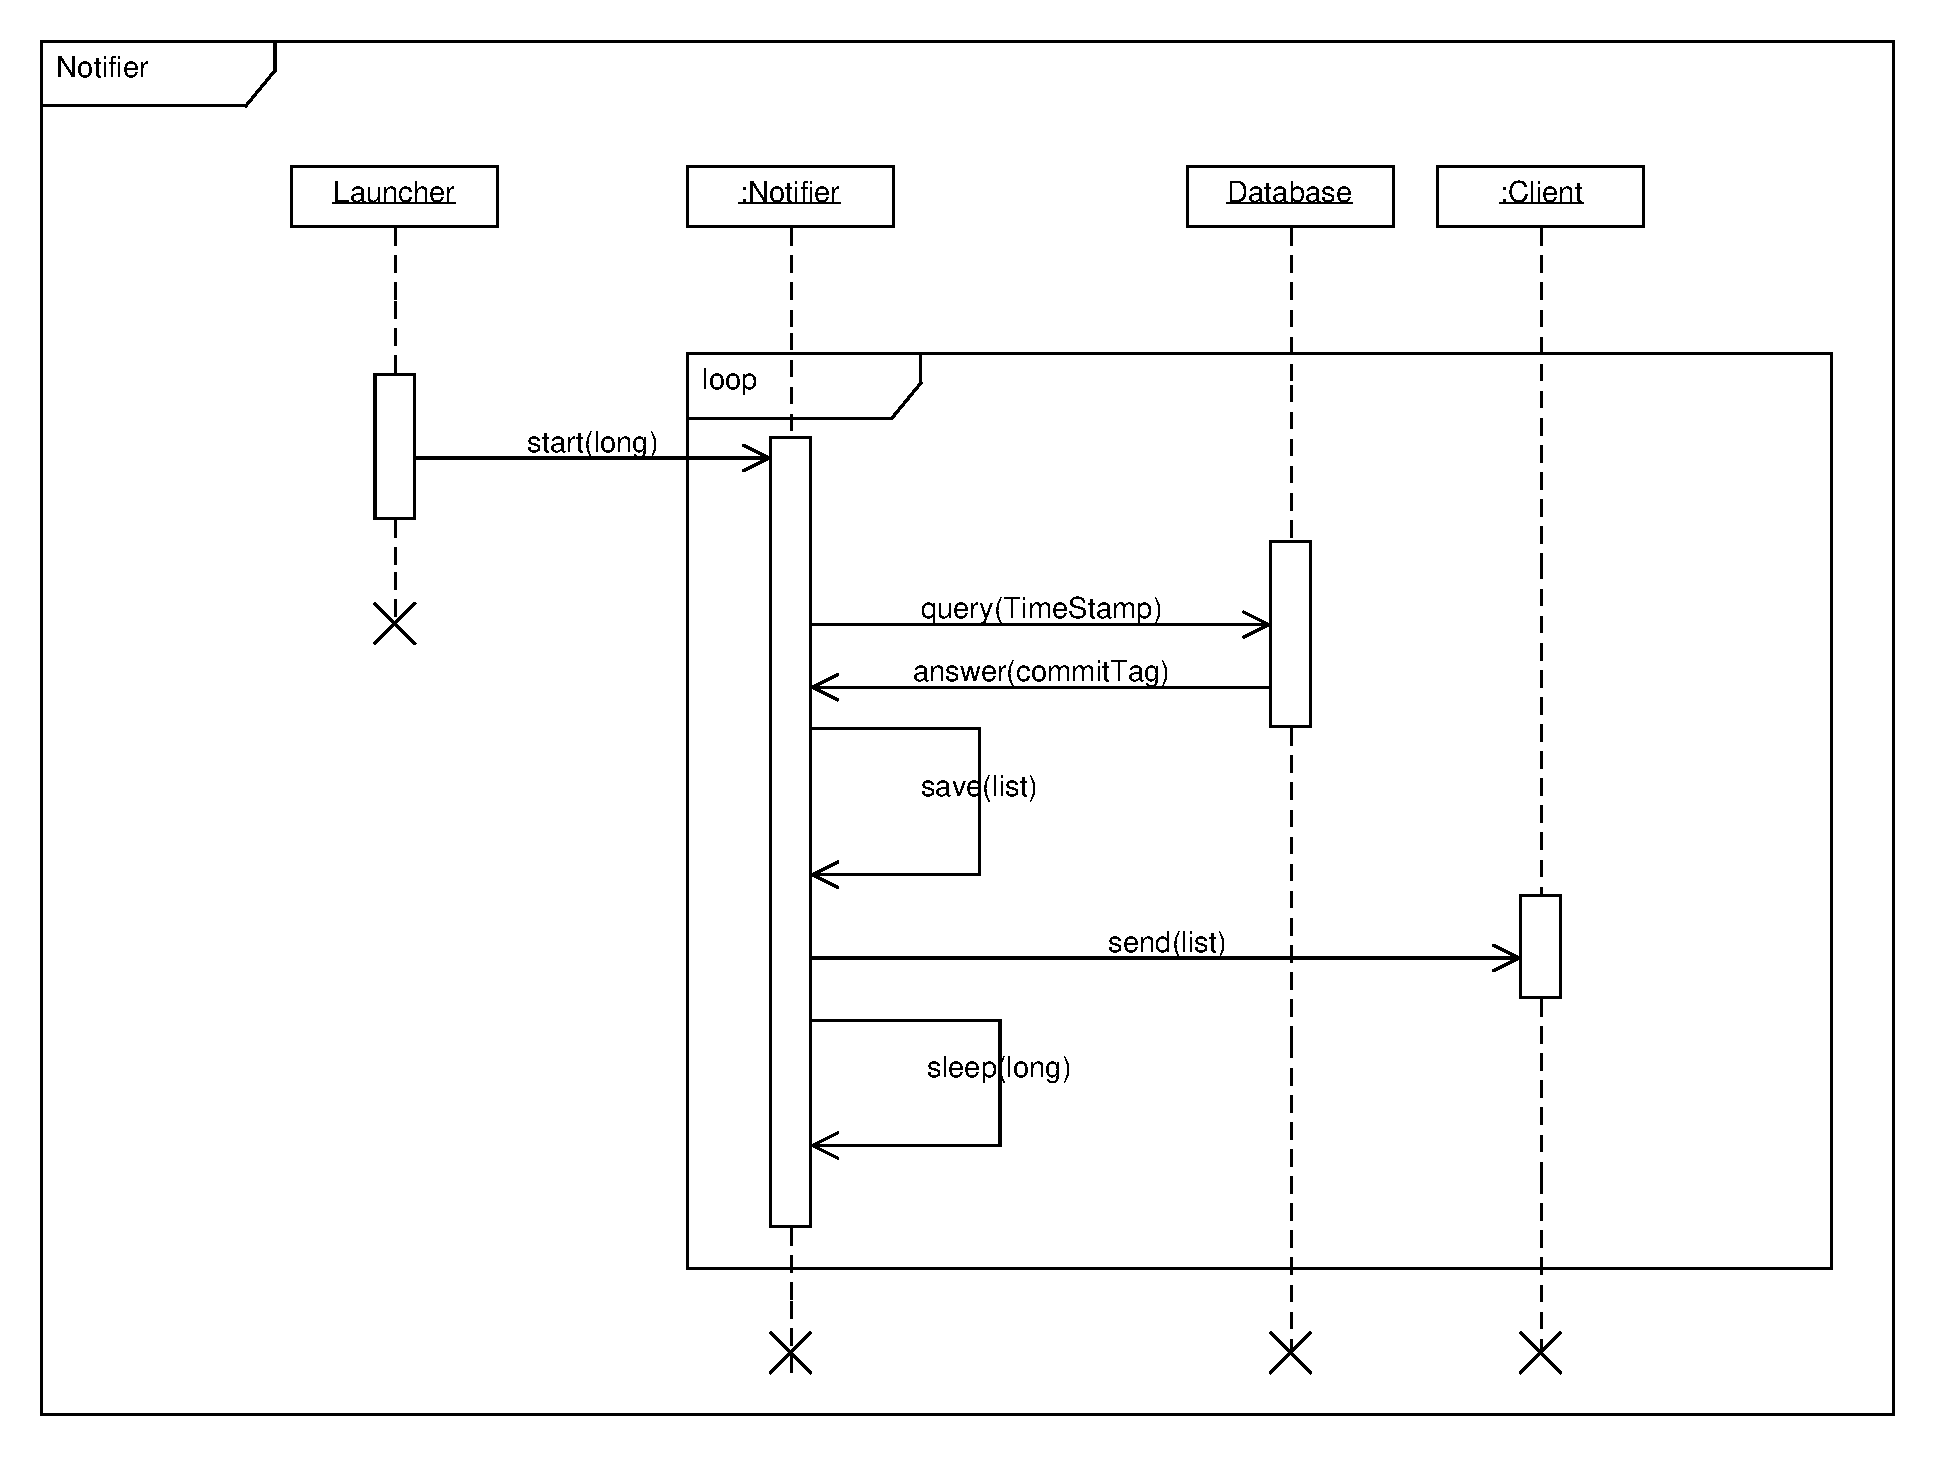
\includegraphics[width=\textwidth]{design/frontend/sequence/notifySequence.pdf}
	\caption{Sequenzdiagramm: Notifier}
\end{figure}
%\subsection {Exception Handling}
%\ref{req:Sv:comm:exceptions}

Sobald Benachrichtigungsroutine mit dem Datum der letzten Suche gestartet wird, macht diese eine Anfrage bei der Datenbank. Als Antwort er hält sie Commit-Tags, welche anschließend in einer Liste zwischengespeichert werden. Danach sendet sie diese Liste an alle Clients. 


\section{Klassen und Komponenten}

\subsection{Server und Client}
\liable{\eddy}
\begin{figure}[H]
	\centering
	\label{dia:design:frontend:classes:svcl}
	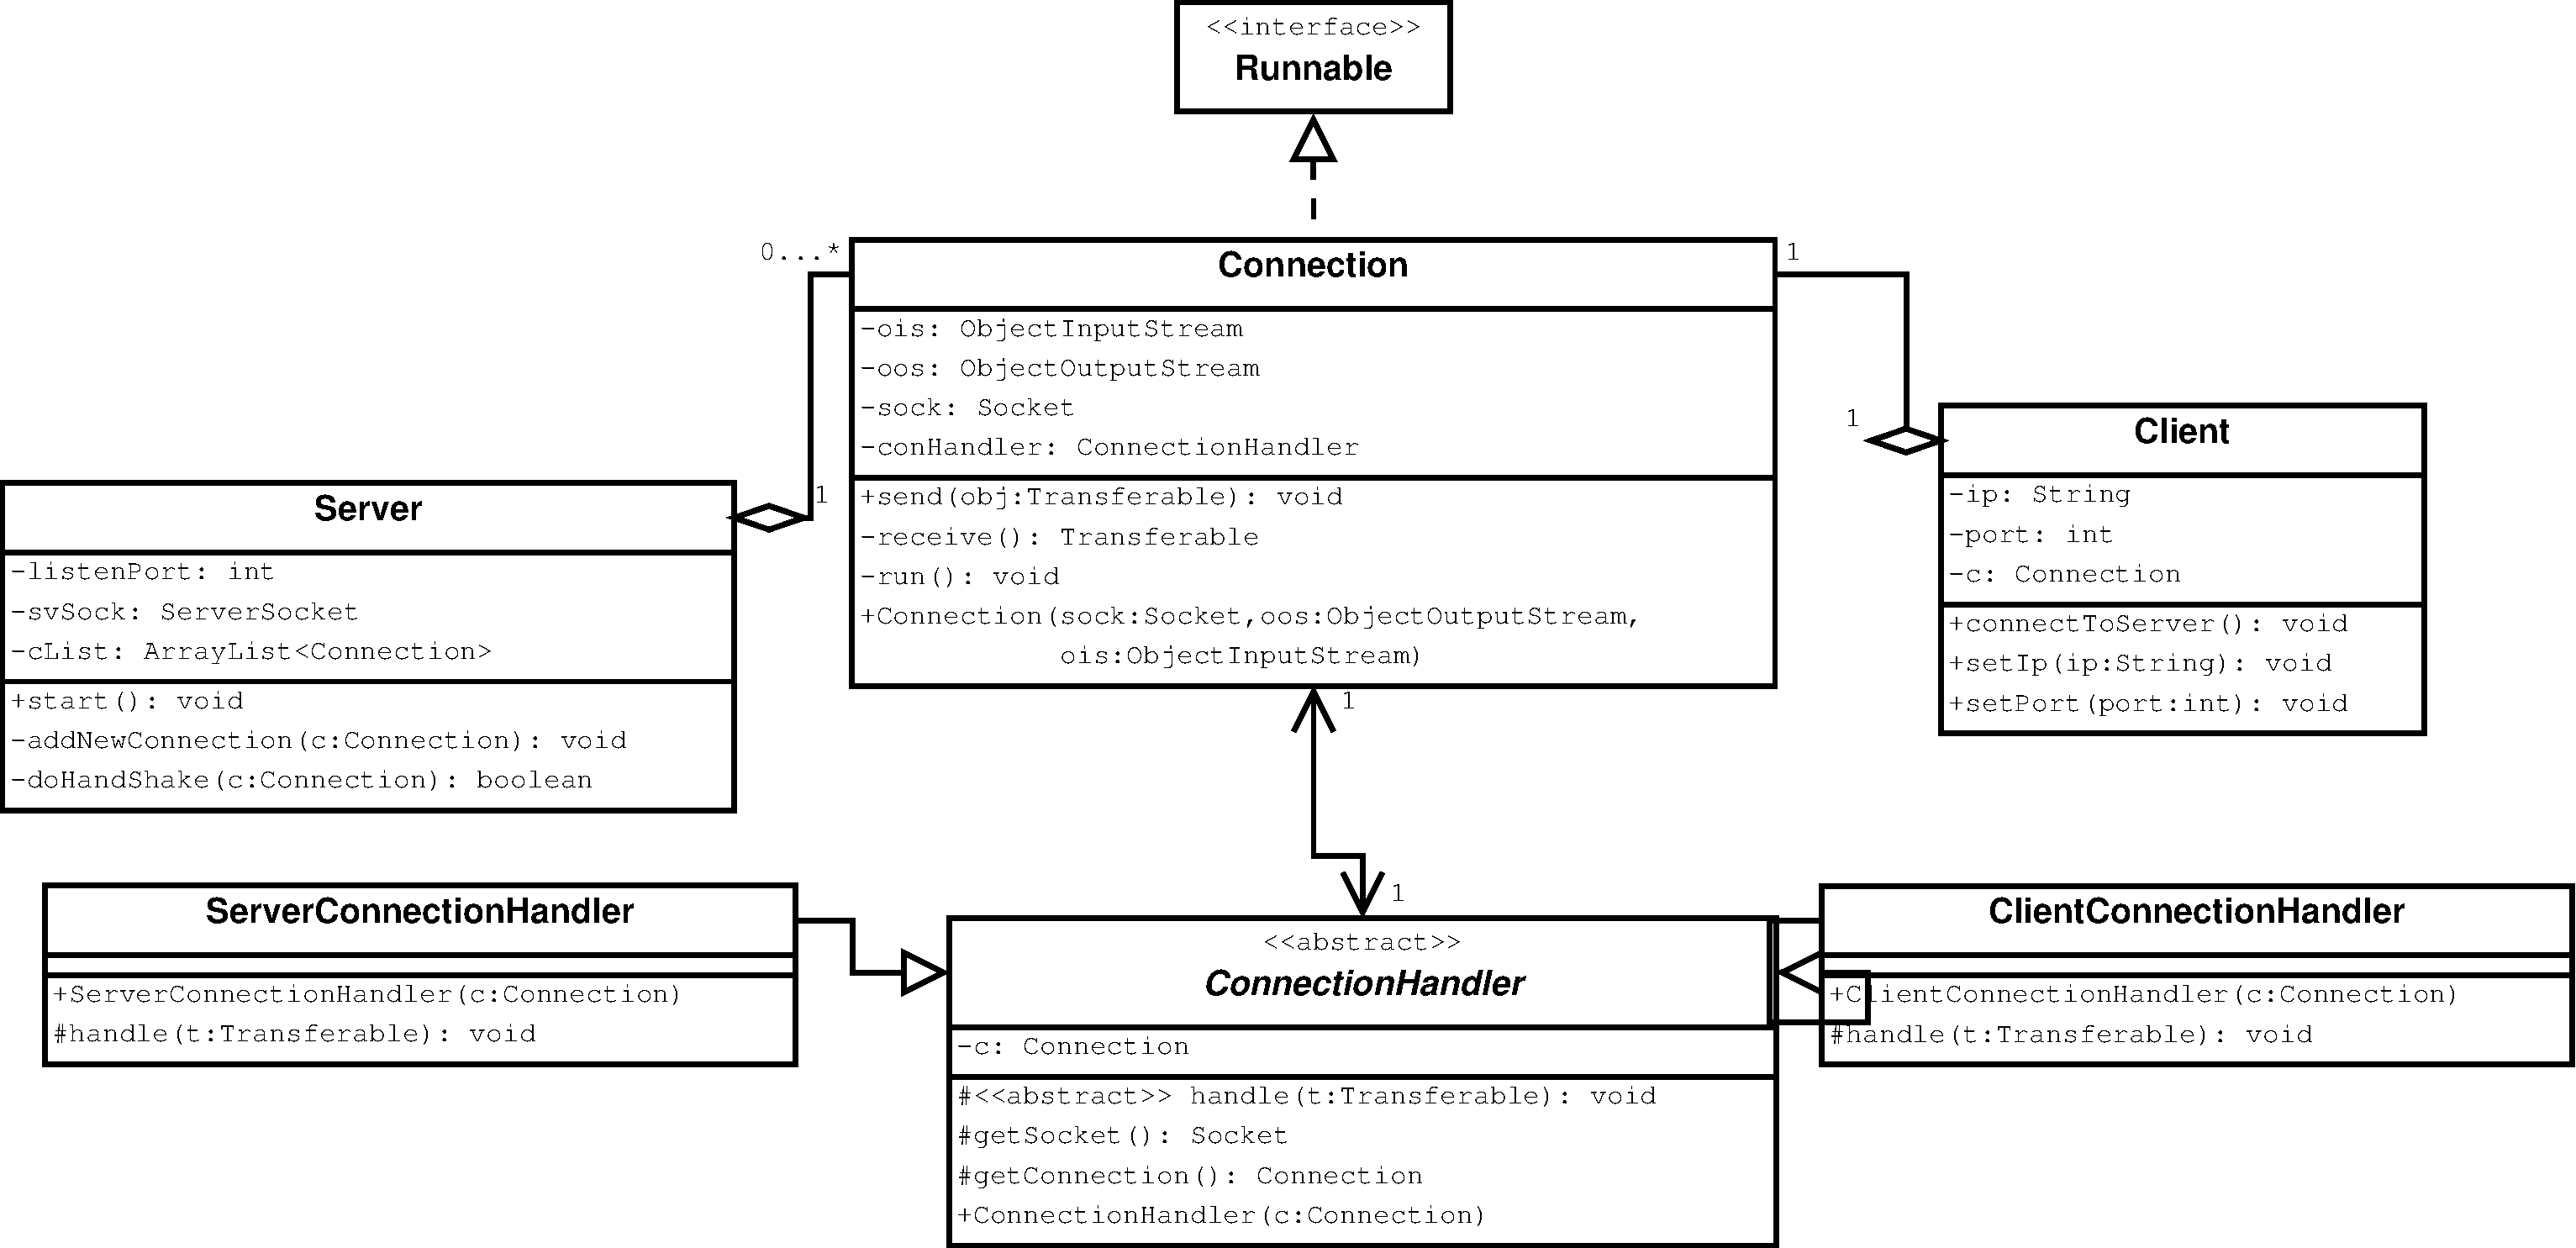
\includegraphics[width=\textwidth]{design/frontend/classes/Server-Client-Klassen.pdf}
	\caption{Klassendiagramm: Server, Client und Connectionhandling}
\end{figure}

\subsection{Messagedaten-Klassen}
\liable{\eddy}

\begin{figure}[H]
	\centering
	\label{dia:design:frontend:classes:datcl}
	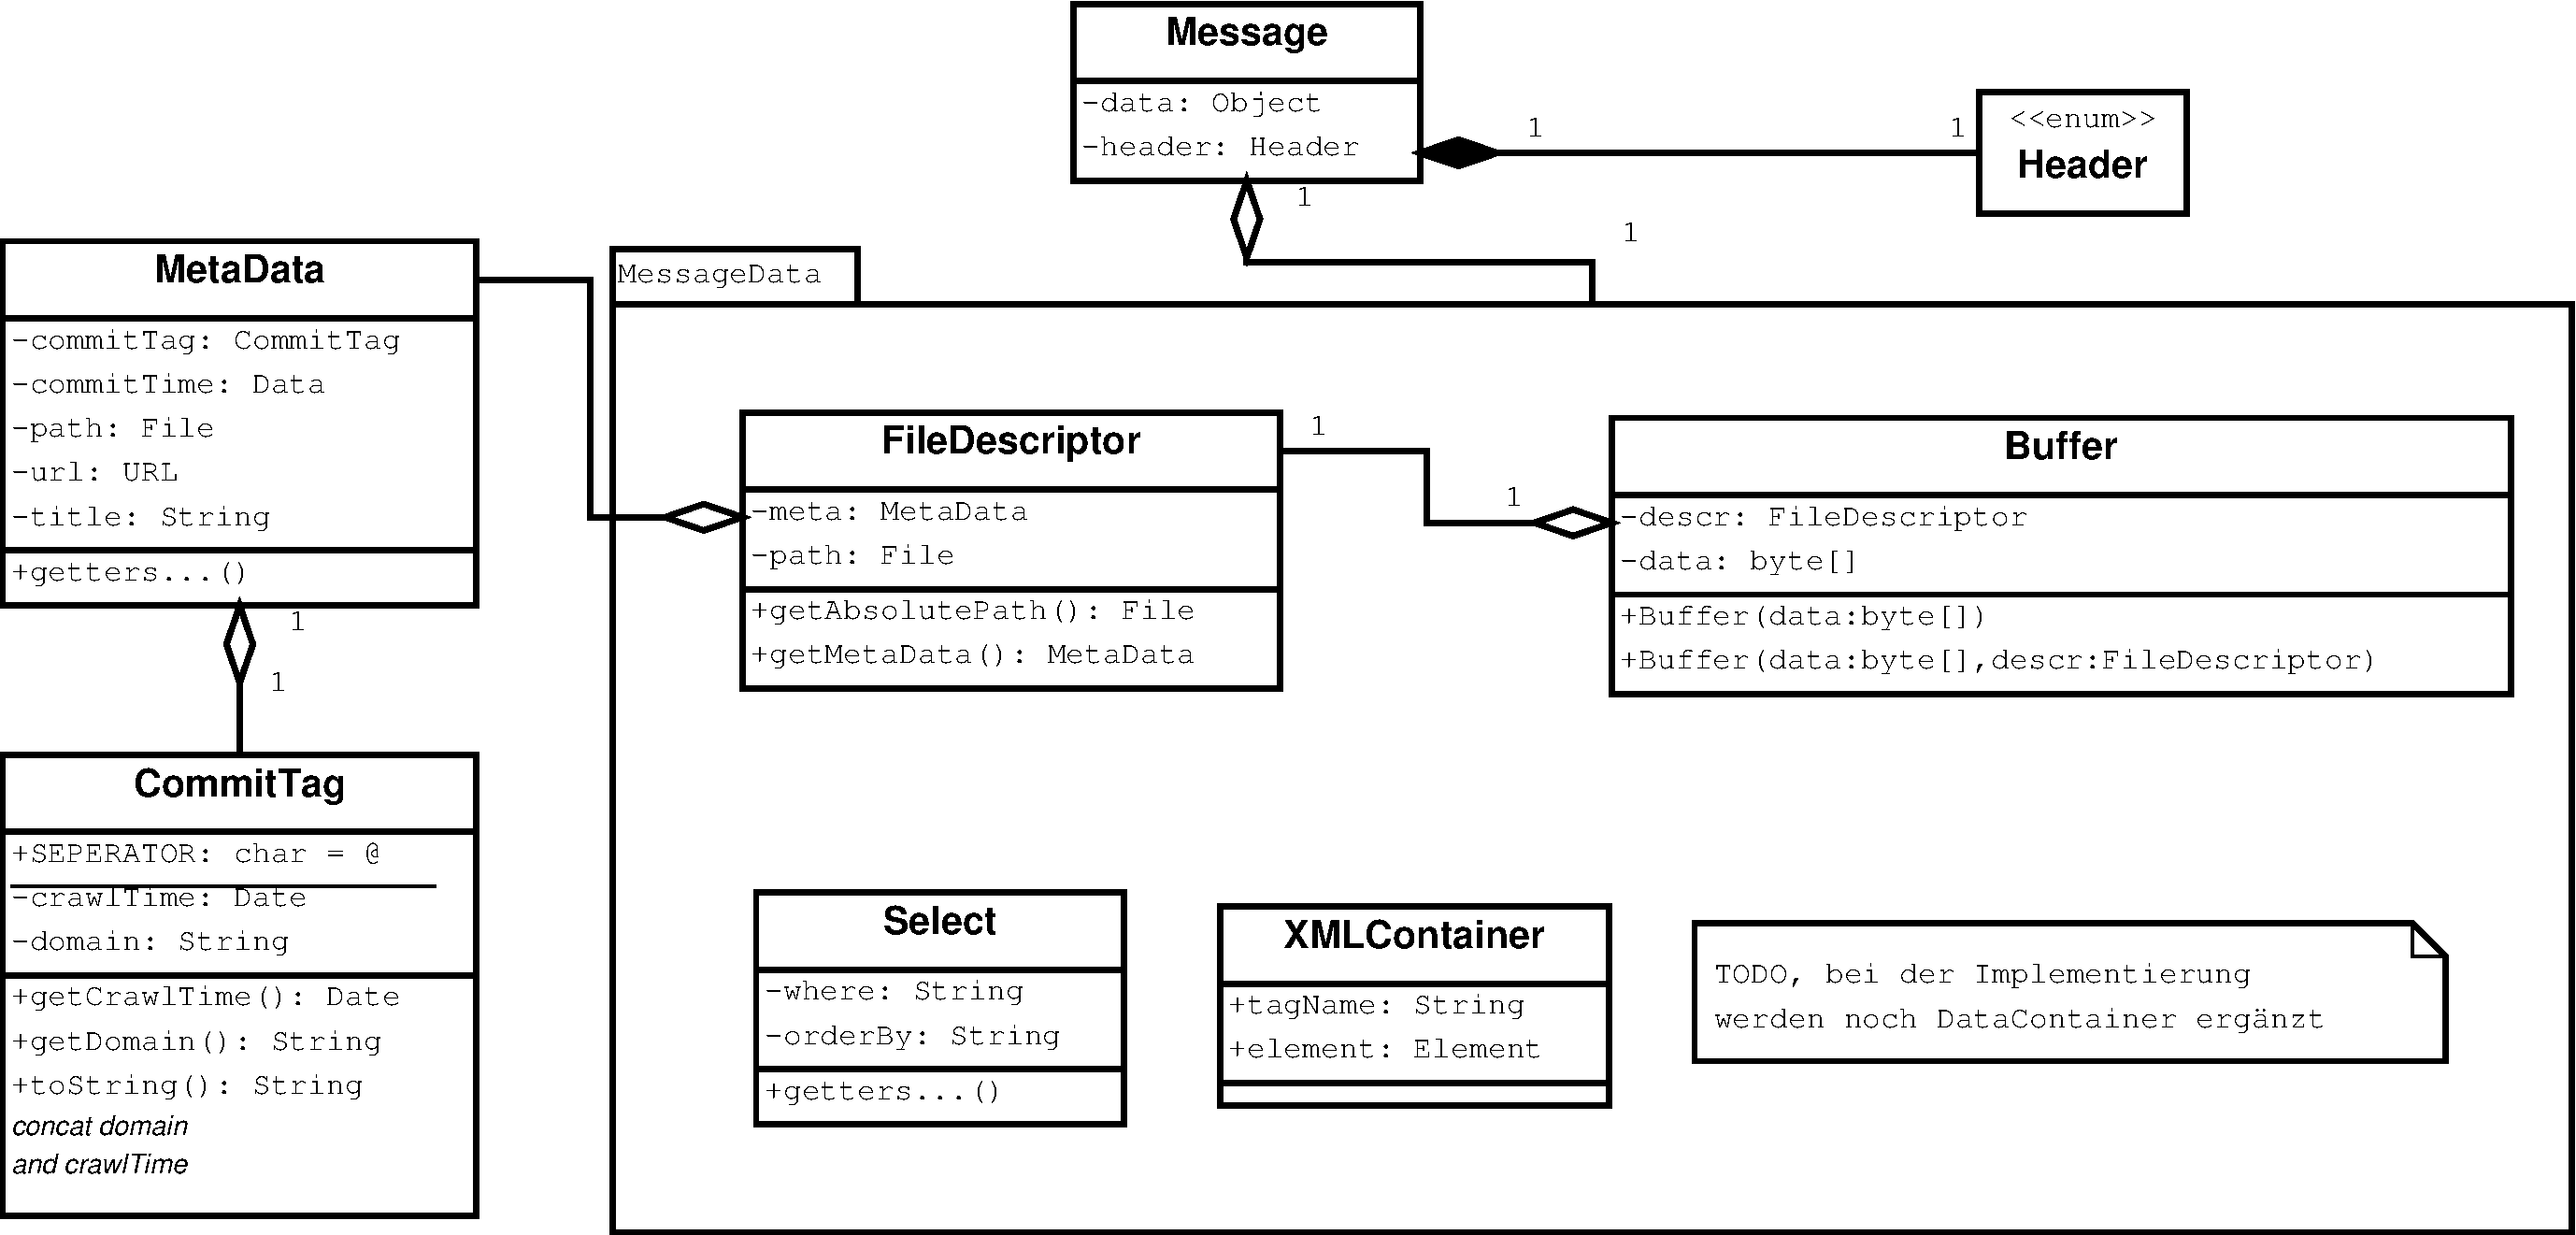
\includegraphics[angle=270, width=.8\textwidth]{design/frontend/classes/MessageDaten-Klassen.pdf}
	\caption{Klassendiagramm: Messagedatenklassen}
\end{figure}

\subsection{Message-Klassen}
\liable{\eddy}

\begin{figure}[H]
	\centering
	\label{dia:design:frontend:classes:msgcl}
	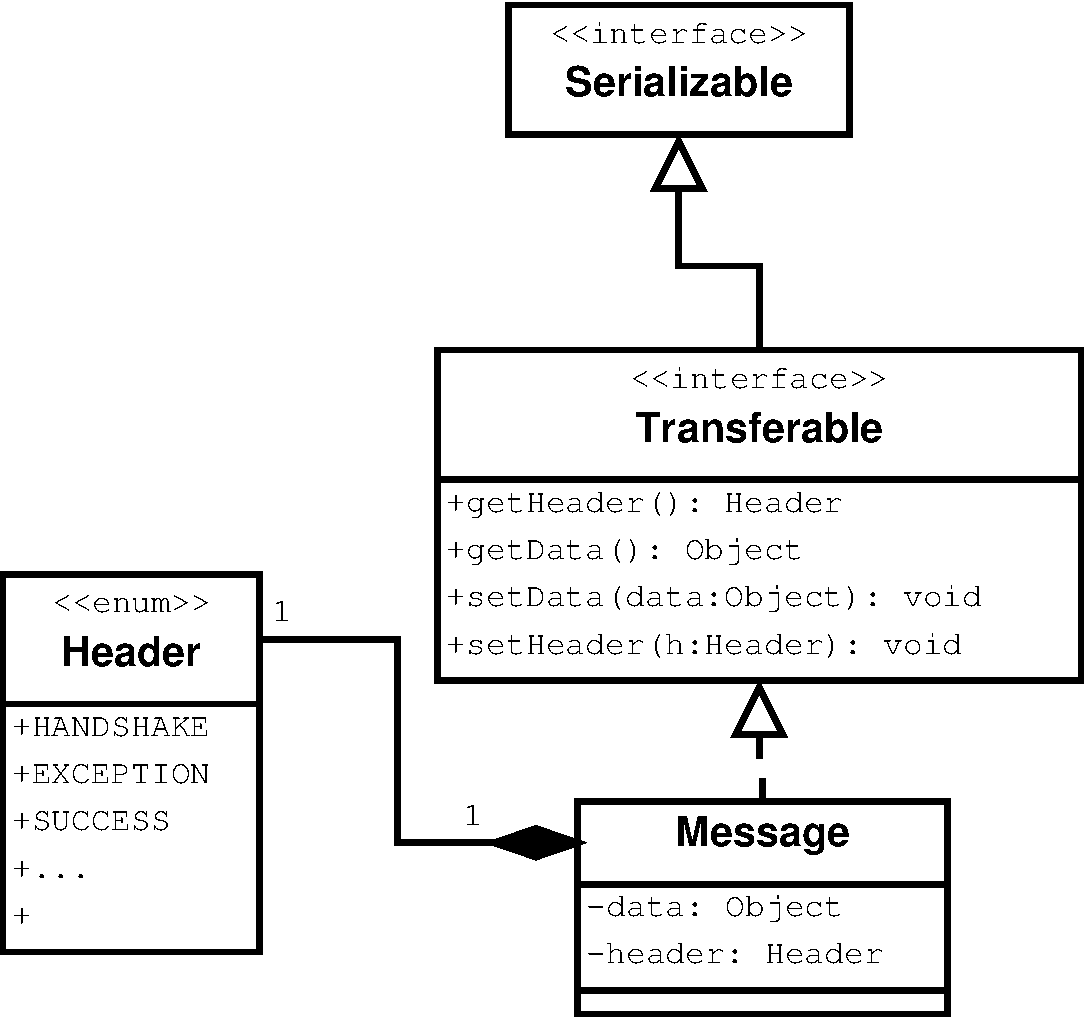
\includegraphics[width=0.5\textwidth]{design/frontend/classes/Message-Klassen.pdf}
	\caption{Klassendiagramm: Datenklassen}
\end{figure}

\subsection{XML-access}
\liable{\cii}
\subsection{Database-access}
\liable{\cii}

\begin{figure}[H]
	\centering
	\label{dia:design:frontend:classes:dbaccess}
	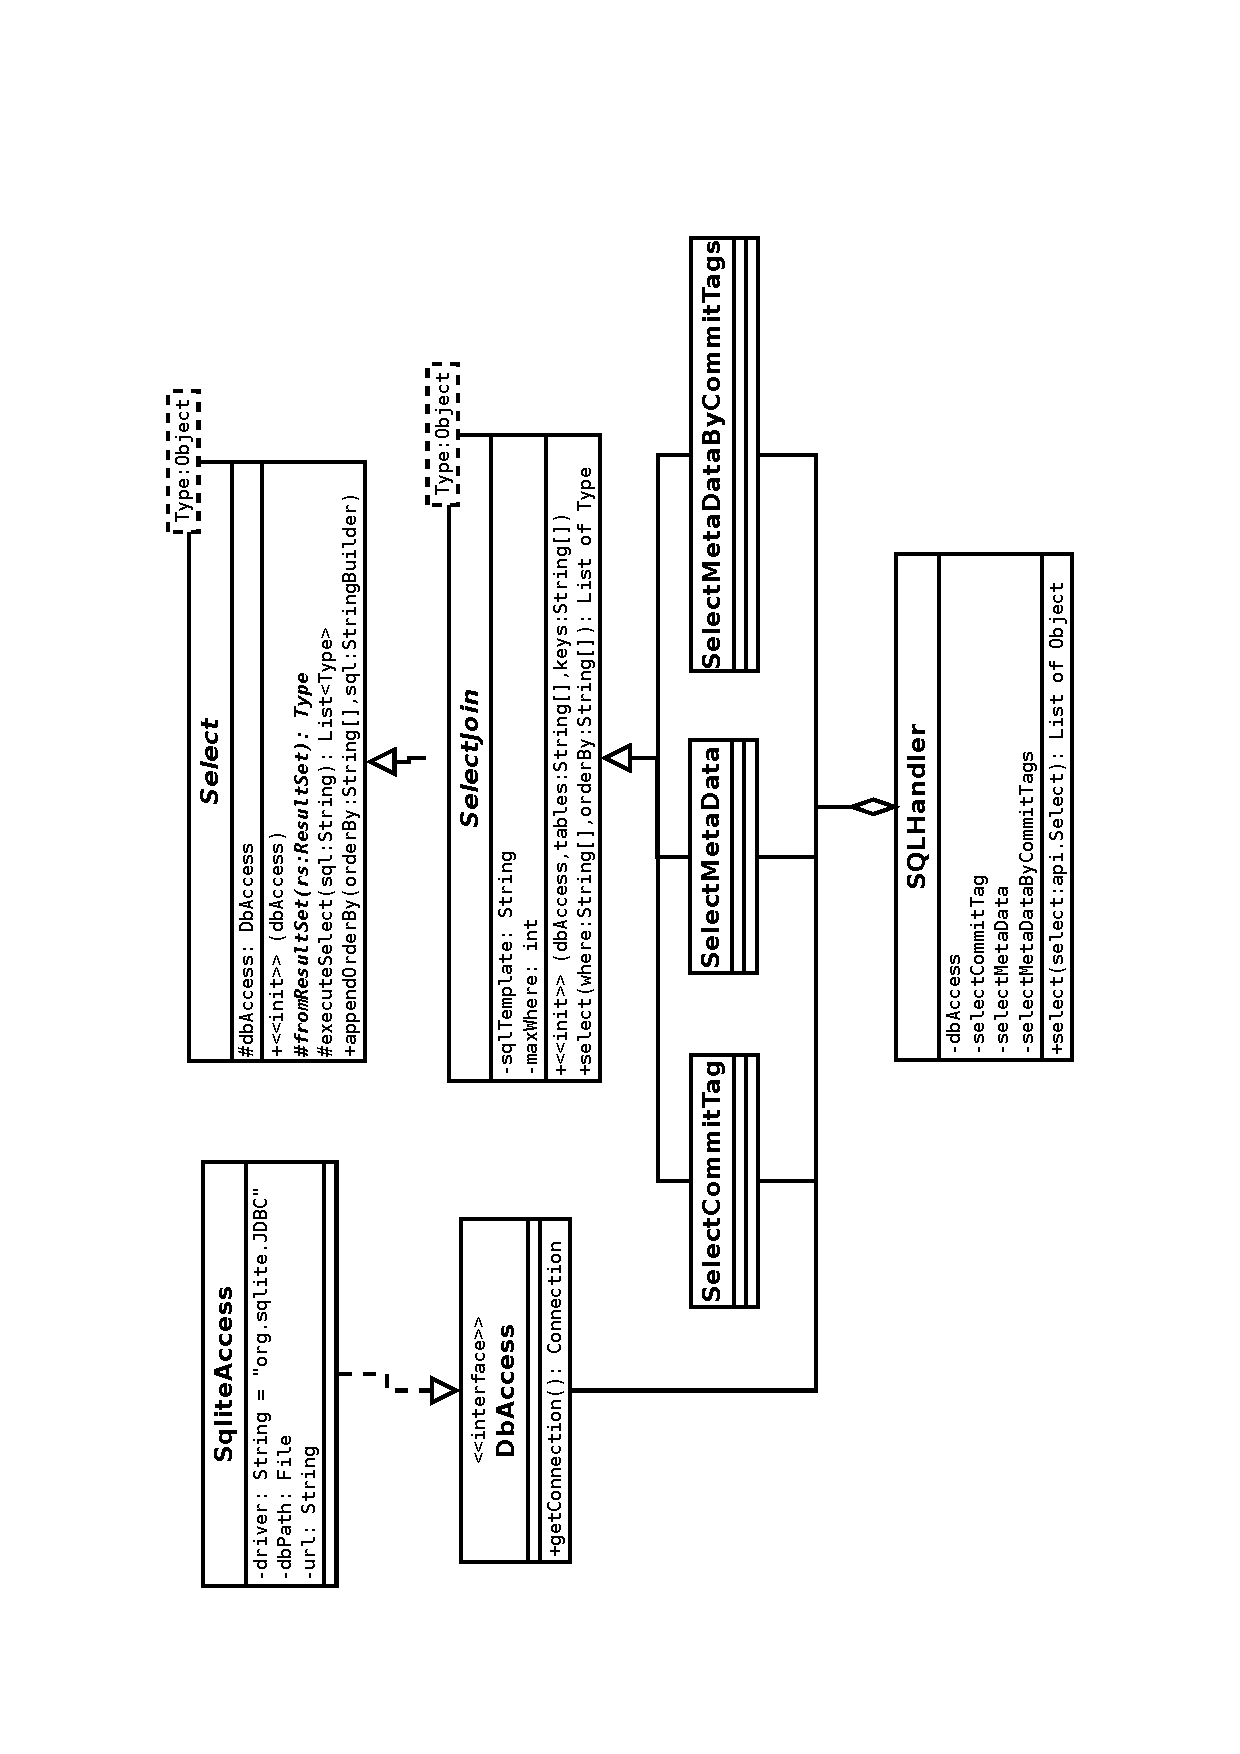
\includegraphics[angle=270, width=1.2\textwidth]{design/frontend/classes/dbaccess-Klassen.pdf}
	\caption{Klassendiagramm: Datenklassen}
\end{figure}

Die dbaccess-Klassen gliedern sich in die folgenden Teile:
\begin{description}
	\item [DbAccess und Ableitungen] kapseln die Verbindung zur Datenbank,
		wobei die Connection für SQLITE implementiert wird.
	\item [SQL-Klassen] diese setzen das Mapping zwischen Objektorientierung und Relationärer Datenbank her, 
		wobei nur SELECT-Statements benötigt werden. 

		Da alle Selects bisher JOINs benötigen, 
		wurde die abstrakte Klasse SelectJoin eingeführt, 
		welche ein vorbereitetes SELECT-JOIN aus mehreren Tabellen zusammenbaut.

		Vom Benutzer übergebenene WHERE und ORDER BY Klauseln können dann dynamisch eingefügt werden. 
		Die so erzeugten SQL-Statements werden dann per JDBC an die Datenbank geschickt und 
		das zurückgegebene ResultSet wird weiterverarbeitet und als Liste des Templatetypen zurückgegeben.
	\item [SqlHandler]
		Der SqlHandler nimmt vom Benutzer erzeugte api.Select-Objekte entgegen, 
		verteilt diese an ein passendes Select-objekt (siehe oben).
\end{description}

\ref{req:Sv:comm}
\section{Test Analysetool} 
\liable{\sab} \\
\ref{req:Cl:testanalyzer} \\
	Das Analysetool wird als einfach Klasse mit main()-funktion implementiert.
	Die Funktion hat den folgenden Ablauf.
	\begin{enumerate}
		\item Es wird ein WebarchiveClient-Objekt erzeugt, über dessen Schnittstellen weitergearbeitet werden kann.
		\item Über ein select() werden einige HTML-Dateien (bekannte Testdaten) aus der Datenbank herausgesucht.
		\item Es wird die Listenschnittstelle benutzt und der Inhalt des Archivordners am Bildschirm ausgegeben.
		\item Mittels der getInputStreamMethode wird die data-Datei geladen.
		\item Diese wird nun ausgelesen und alle Wörter gezählt. Der Einfachheit halber wird alles als Wort angesehen, was durch whitespace getrennt ist.
		\item Das Ergebnis wird mittels  getOutputStream in eine Textdatei auf dem Archiv geschrieben.
		\item Zusätzlich wird das Ergebnis als neues Element in die XML-Begleitdatei geschrieben.
			Dazu muss vorher ein XMLEdit-objekt vom Client angefordert werden.
	\end{enumerate}
		
